% Use only LaTeX2e, calling the article.cls class and 12-point type.


\documentclass[12pt]{article}

% Users of the {thebibliography} environment or BibTeX should use the
% scicite.sty package, downloadable from *Science* at
% www.sciencemag.org/about/authors/prep/TeX_help/ .
% This package should properly format in-text
% reference calls and reference-list numbers.
\usepackage{cite}
\usepackage{graphicx}


% Use times if you have the font installed; otherwise, comment out the
% following line.

\usepackage{times,graphicx}

% The preamble here sets up a lot of new/revised commands and
% environments.  It's annoying, but please do *not* try to strip these
% out into a separate .sty file (which could lead to the loss of some
% information when we convert the file to other formats).  Instead, keep
% them in the preamble of your main LaTeX source file.


% The following parameters seem to provide a reasonable page setup.

\topmargin 0.0cm
\oddsidemargin 0.2cm
\textwidth 16cm 
\textheight 21cm
\footskip 1.0cm


%The next command sets up an environment for the abstract to your paper.

\newcommand{\roots}  {\ensuremath{\sqrt{s}}}
\newcommand{\rootsNN}  {\ensuremath{\sqrt{s_{_{NN}}}}}
\newcommand{\pp}{\ensuremath{\text{pp}}\xspace}
\newcommand{\pPb}{\ensuremath{\text{pPb}}\xspace}
\newcommand{\dphi}     {\ensuremath{\Delta\phi}}
\newcommand{\noff}    {\ensuremath{N_\text{trk}^\text{offline}}\xspace}
\newcommand{\non}    {\ensuremath{N_\text{trk}^\text{online}}\xspace}
\newcommand {\deta}     {\ensuremath{\Delta\eta}}
\newcommand {\AonA}  {\ensuremath{\text{AA}}\xspace}
\newcommand {\pA}    {\ensuremath{\text{pA}}\xspace}
\newcommand {\PbPb}  {\ensuremath{\text{PbPb}}\xspace}
\newcommand {\CuCu}  {\ensuremath{\text{CuCu}}\xspace}
\newcommand {\AuAu}  {\ensuremath{\text{AuAu}}\xspace}
\newcommand {\dAu}  {\ensuremath{\text{dAu}}\xspace}
\newcommand{\mubinv} {\ensuremath{\,\mu\mathrm{b}^{-1}}\xspace}
\newcommand{\mum} {\ensuremath{\,\mu\mathrm{m}}\xspace}
\newcommand{\pt}       {\ensuremath{p_\mathrm{T}}}
\newcommand{\Et}       {\ensuremath{E_\mathrm{T}}}
\newcommand {\pta}       {\ensuremath{p_\mathrm{T}^{\mathrm{a}}}}
\newcommand {\ptb}       {\ensuremath{p_\mathrm{T}^{\mathrm{b}}}}
\newcommand {\etaa}       {\ensuremath{\eta^{\mathrm{a}}}}
\newcommand {\etab}       {\ensuremath{\eta^{\mathrm{b}}}}
\newcommand{\HYDJET} {\textsc{hydjet}\xspace}
\newcommand{\AMPT} {\textsc{ampt}\xspace}
\newcommand{\HIJING} {\textsc{hijing}\xspace}

\newenvironment{sciabstract}{%
\begin{quote} \bf}
{\end{quote}}


% If your reference list includes text notes as well as references,
% include the following line; otherwise, comment it out.

\renewcommand\refname{References and Notes}

% The following lines set up an environment for the last note in the
% reference list, which commonly includes acknowledgments of funding,
% help, etc.  It's intended for users of BibTeX or the {thebibliography}
% environment.  Users who are hand-coding their references at the end
% using a list environment such as {enumerate} can simply add another
% item at the end, and it will be numbered automatically.

\newcounter{lastnote}
\newenvironment{scilastnote}{%
\setcounter{lastnote}{\value{enumiv}}%
\addtocounter{lastnote}{+1}%
\begin{list}%
{\arabic{lastnote}.}
{\setlength{\leftmargin}{.22in}}
{\setlength{\labelsep}{.5em}}}
{\end{list}}


% Include your paper's title here

\title{CMS perspectives on the pPb run in 2016} 


% Place the author information here.  Please hand-code the contact
% information and notecalls; do *not* use \footnote commands.  Let the
% author contact information appear immediately below the author names
% as shown.  We would also prefer that you don't change the type-size
% settings shown here.

\author
{ The CMS Collaboration }

% Include the date command, but leave its argument blank.

\date{}

%%%%%%%%%%%%%%%%% END OF PREAMBLE %%%%%%%%%%%%%%%%



\begin{document} 

% Double-space the manuscript.

\baselineskip24pt

% Make the title.

\maketitle 

% Place your abstract within the special {sciabstract} environment.

\begin{abstract}

This note presents CMS perspectives on the pPb run in 2016 at the LHC. 
Physics motivations and corresponding integrated luminosity required are discussed.


%The first ridge discovery in p-p is here: Ref.~\cite{Khachatryan:2010gv}

\end{abstract}

\section*{Introduction}

pPb run with integrated luminosity of 35 nb$^{-1}$ has been collected.
nuclear parton distribution function (nPDF)

It has been decided in 2016 that the heavy ion run will be splitted between 5 and 8 TeV.

\begin{itemize}
\item Is a QGP fluid formed in pPb collisions?
\item Explore nPDF over unexplored regime in x and Q.
\end{itemize}

We need integrated luminosity as high as possible. 
We use 100 nb$^{-1}$ as a demonstration.
\section{QGP fluid in small systems}

\begin{figure}[thb]
  \begin{center}
    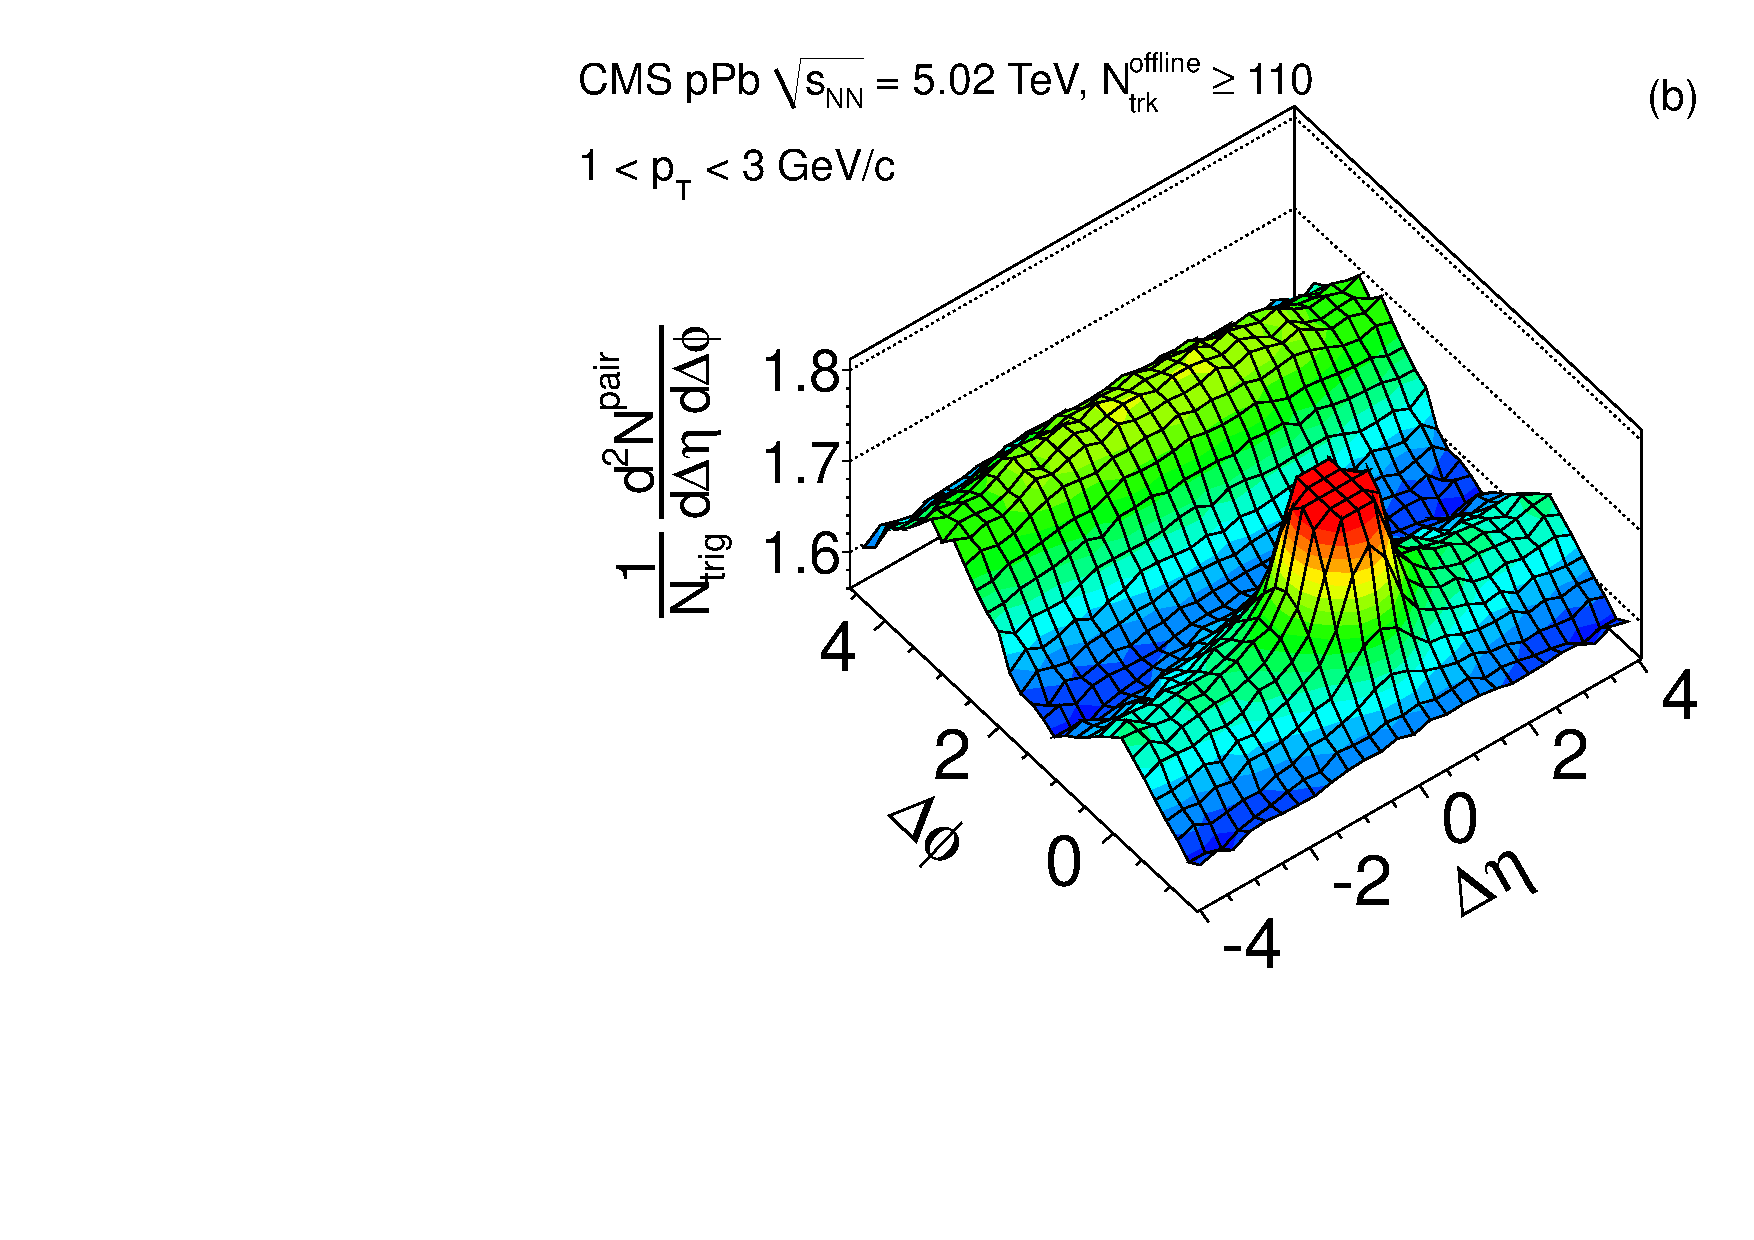
\includegraphics[width=0.48\textwidth]{figures/corr2D_pPb_N110_pt1-3_20121016.pdf}
    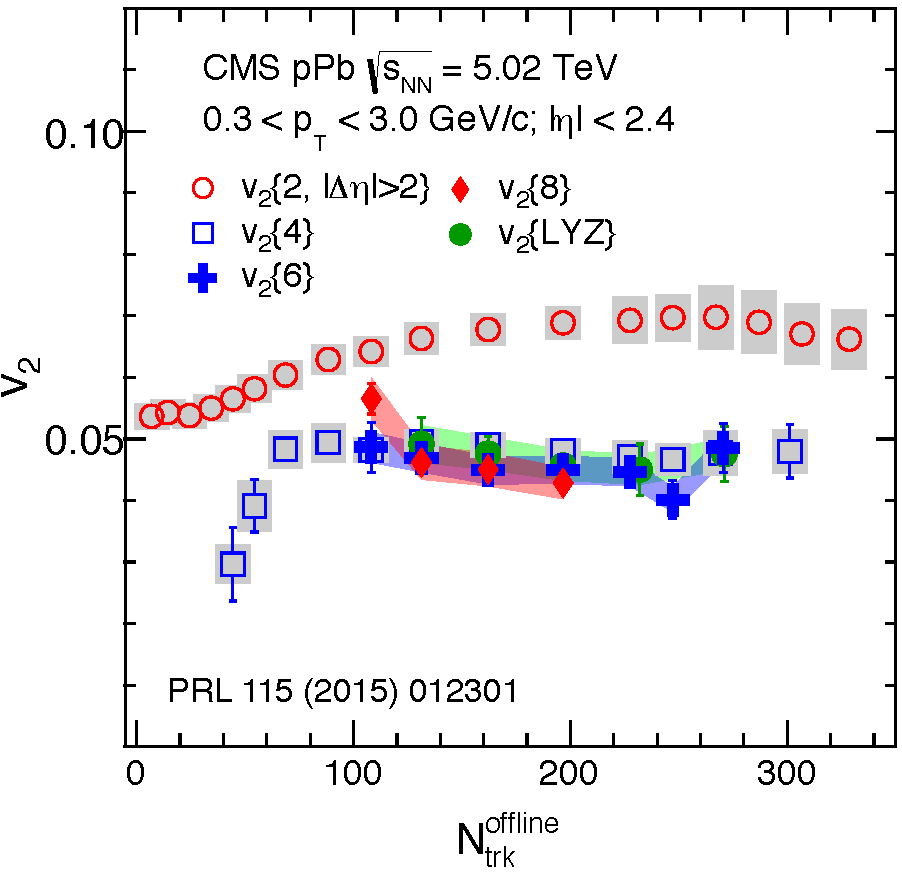
\includegraphics[width=0.48\textwidth]{figures/v2m_pPb.pdf}
    \caption{ Left: The 2D two-particle correlation functions in high-multiplicity 
    pPb collisions at \rootsNN\ = 5.02 TeV measured by the CMS experiment.
    Right: The elliptic anisotropy, $v_2$, as a function of $N_{\rm trk}$
    obtained from two-, four-, six- and eight-particle cumulants, and the LYZ method, 
    averaged over $0.3<\pt<3.0$~GeV/c, in pPb collisions at \rootsNN\ = 5.02 TeV.
  %~\cite{Khachatryan:2015waa}.
    }
    \label{fig:ridge_pPb}
  \end{center}
\end{figure} 

Observation of a long-range, near-side structure (often called the ``Ridge'') in two-particle
\deta\ -- \dphi\ correlation function of high-multiplicity pp~\cite{Khachatryan:2010gv} 
and pPb~\cite{CMS:2012qk} collisions at CMS (Fig.~\ref{fig:ridge_pPb} left)
opened up new opportunities for studying novel dynamics of particle production 
in small but high-density Quantum Chromodynamic (QCD) systems. Similar ridge-like structure is
first observed in relativistic nucleus-nucleus (AA) collisions, and is widely accepted 
to be originated from the hydrodynamic collective flow of a strongly interacting and 
expanding medium. 

In small colliding systems like pp and pPb, there has not been a consensus yet
in the community on the origin of the ridge-like correlation structure. 
While the formation of a hot and dense fluid-like medium provides a natural explanation, 
it was not expected because the overlapping region is significantly smaller than 
that in an AA collision. Various alternative theoretical interpretations have been 
proposed, such as models of initial-state gluon correlations without any final-state interactions.
A key observation made by CMS in 2013 pPb run at \rootsNN\ = 5.02 TeV is that
the elliptic azimuthal anisotropy harnomics, $v_2$, extracted using four-, six-,
eight- and all particle azimuthal correlations, are found to be nearly identical
within about 10\%~\cite{Khachatryan:2015waa}, lending strong support to the highly 
collective nature of correlations in these systems. 

While much progress has been made in the LHC run 1, many questions still remain unanswered:
(1) What is the underlying mechanism driving the observed collective behavior of particles? 
Strong final-state rescatterings in an initially eccentric system (like AA collisions) or 
initial momentum-space correlations due to initial-state gluon interactions? (2) If a hot and opaque 
medium is indeed formed in a pPb collision, how does it influence the behavior of hard probes
such as jets and quarkonia? Higher energy and luminosity pPb collisions at the LHC run 2 
will enable a wide range of high precision measurements, providing us unique opportunities 
to address these important questions. 
\subsection{Collectivity and Flow}

An important point that should be kept in mind is that the very events
showing strong collectivity in small systems are in a class of their own.
They represent a small fraction of the total cross-section with highest particle
multiplicities produced. Events with 100--200 tracks (these are the high-multiplicity 
events where a ridge signal is seen in pp and pPb) are a common occurrence in
PbPb collisions but rare in pPb collisions, thus questing for high-luminosity data samples.

\begin{figure}[t!]
  \begin{center}
    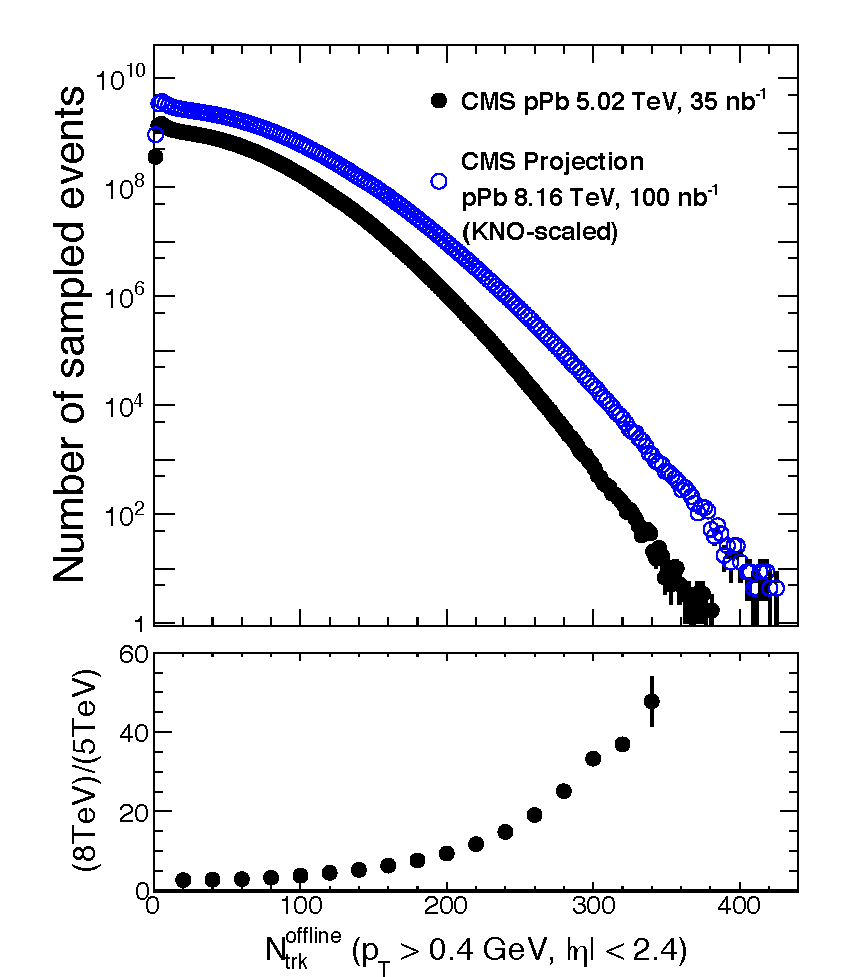
\includegraphics[width=0.6\textwidth]{figures/Ntrk.pdf}
    \caption{ Projected charged particle multiplicity distribution for pPb 
    collisions at \rootsNN\ = 8.16 TeV with L$_{\rm int}$ = 100 nb$^{-1}$
    based on the KNO scaling of measured distribution at \rootsNN\ = 5.02 TeV.
    }
    \label{fig:Ntrk_pPb}
  \end{center}
\end{figure}

Based on an approximate KNO scaling of multiplicity distribution at different collision 
energies, a projection of multiplicity distribution for pPb collisions at \rootsNN\ = 8.16 
TeV is presented in Fig.~\ref{fig:Ntrk_pPb}, corresponding to an integrated luminosity 
of 100 nb$^{-1}$. A ratio of multiplicity distributions at \rootsNN\ = 8.16 TeV 
to \rootsNN\ = 5.02 TeV (L$_{\rm int}$ = 35 nb$^{-1}$) is also shown in the bottom panel of Fig.~\ref{fig:Ntrk_pPb} (Note that the KNO scaling is known to be not exact so the ratio 
is likely to be a little underestimated, especially at large $N_{\rm trk}$ values). 
As one can see, significant enhancement in high-multiplicity event sample is expected 
in 2016 pPb run. The enhancement factor increases as a function of multiplicity owing 
to the increase of collision energy. For instance at $N_{\rm trk}$ value $\approx$ 250, 
20 times more events are expected comparing to 2013 pPb data sample at \rootsNN\ = 5.02 TeV
(a factor of 7 from higher collision energy).

\begin{figure}[t!]
  \begin{center}
    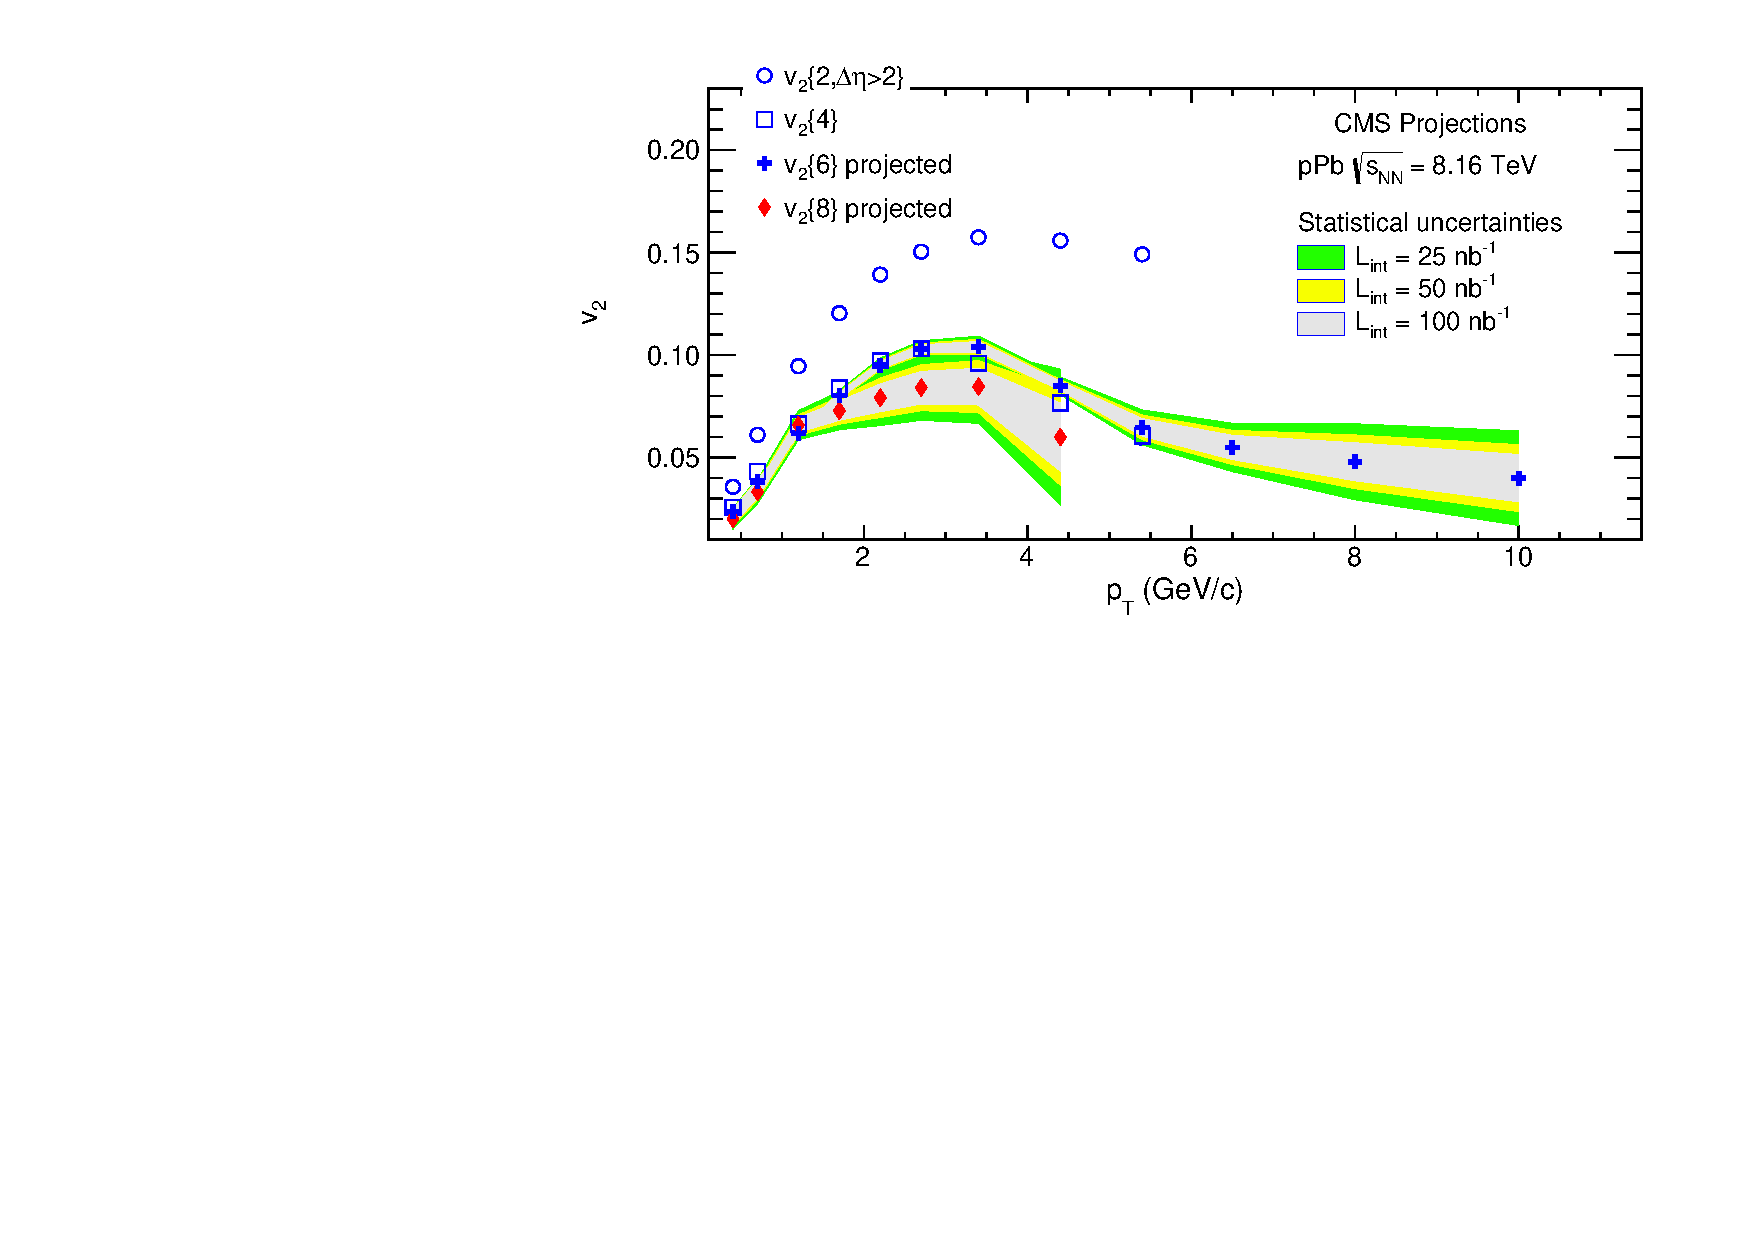
\includegraphics[width=\textwidth]{figures/vnpT_proj_100nb_combineLumi.pdf}
    \caption{ Projected statistical uncertainties of $v_2\{6\}$ and $v_2\{8\}$ as a function of \pt\ 
    for pPb collisions at \rootsNN\ = 8.16 TeV, based on data at \rootsNN\ = 5.02 TeV, with luminosity
    scenarios of L$_{\rm int}$ = 100, 50 and 25 nb$^{-1}$. Data points for $\pt<6$ GeV/c
    are directly taken from 5.02 TeV measurement while $v_{2}\{6\}$ values for $\pt>6$ GeV/c
    are hypothetical, mainly for demonstrating the statistical sensitivity at very high \pt.
    }
    \label{fig:vnpT}
  \end{center}
\end{figure}

Following the observation of collectivity for $\pt$-inclusive 
particles~\cite{Khachatryan:2015waa} (Fig.~\ref{fig:ridge_pPb}, right), 
a natural question to pursue is whether this collectivity extends differentially 
in particle \pt\ to higher \pt\ regime. First attempt has been 
made using run-1 pPb data, where $v_2$ is measured 
by correlating one particle at different \pt\ with multiple low-\pt\ particles 
($0.3<\pt<3$ GeV/c) in high-multiplicity pPb collisions~\cite{CMS-PAS-HIN-15-008}.
Due to statistical limitation, it is not possible to conclude on the relation of $v_{2}$
values extracted from four-, six- and eight-particle correlations as a function of \pt.

Figure~\ref{fig:vnpT} shows the projected statistical precision for $v_{2}\{6\}$
and $v_{2}\{8\}$ as a function of \pt\ that can be achieved in 2016 pPb run at 
\rootsNN\ = 8.16 TeV. Three different integrated luminosity scenarios of L$_{\rm int}$ = 
100, 50 and 25 nb$^{-1}$ are presented. Data points for $\pt<6$ GeV/c are directly 
taken from 5.02 TeV measurement, while $v_{2}\{6\}$ values for $\pt>6$ GeV/c are 
hypothetical, mainly for demonstrating the statistical sensitivity at very high \pt.
With L$_{\rm int}$ = 100 nb$^{-1}$, the collective nature of particle production 
is expected to be well constrained up to \pt\ about 6 GeV/c.
The $v_2$ value from six-particle correlations can be even explored to \pt\ around 10 GeV/c, 
a regime dominated by hard QCD processes. Observation of a finite $v_2$ value at very 
high \pt, especially via multiparticle correlations, would be indicative 
of medium interactions with hard partons in pPb collisions. A reduced data sample
of, e.g., L$_{\rm int}$ = 50 or 25 nb$^{-1}$ would significantly compromise 
the goal of exploring this exciting physics, as illustrated in the figure.

\begin{figure}[t!]
  \begin{center}
    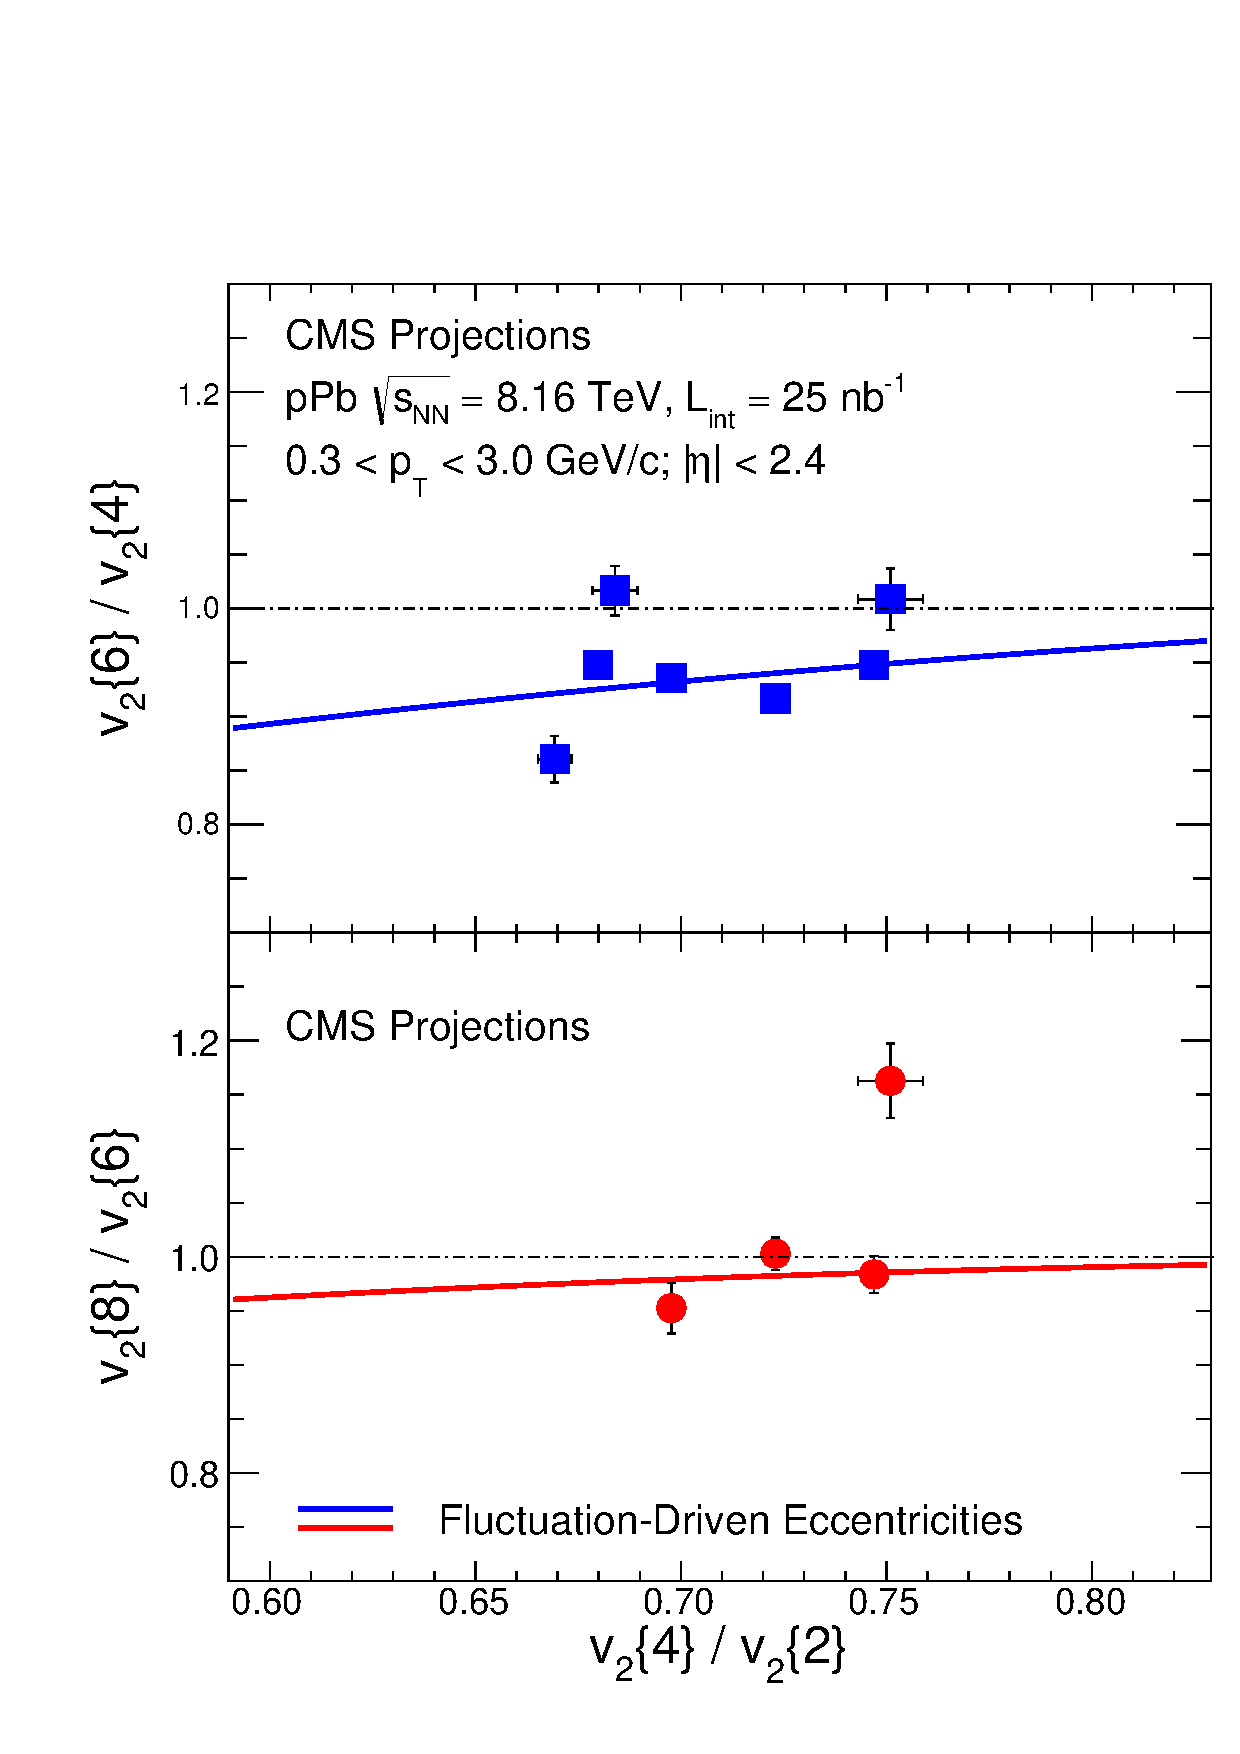
\includegraphics[width=0.5\textwidth]{figures/vnRatios_proj_100nb.pdf}
    \caption{ Projected statistical uncertainties of $v_2\{4\}/v_2\{2\}$, $v_2\{6\}/v_2\{4\}$ and $v_2\{8\}/v_2\{6\}$ ratios
    for pPb collisions at \rootsNN\ = 8.16 TeV with L$_{\rm int}$ = 100 nb$^{-1}$, based on data at \rootsNN\ = 5.02 TeV.
    }
    \label{fig:vnNtrk}
  \end{center}
\end{figure}

Once the collective nature of particle production is established, 
the next question to address is what the underlying mechanism is in 
driving the collectivity. Specifically, the goal of CMS is to 
disentangle different proposed theoretical scenarios such as hydrodynamic models and
gluon saturation models via high precision measurements. 

Hydrodynamic model predicts that $v_2$ is proportional to the 
eccentricity, $\epsilon_{2}$, of the initial colliding system.
Based on initial-state eccentricity fluctuations, a quantitative
relationship among $v_2\{2\}$, $v_2\{4\}$, $v_2\{6\}$ and $v_2\{8\}$ 
has been predicted, denoted as solid curves in Fig.~\ref{fig:vnNtrk}~\cite{Yan:2013laa}. 
While the values of $v_2\{4\}$, $v_2\{6\}$ and $v_2\{8\}$
are expected to be very similar, a few \% deviation is expected in the context of
hydrodynamic scenario. Such a small deviation has been explored in 2013 
pPb run~\cite{Khachatryan:2015waa}. An indication of data being consistent 
with hydrodynamic prediction is seen but it remains inconclusive due to 
statistical limitation. In Fig.~\ref{fig:vnNtrk}, based on the 2013 pPb data, the projected statistical
uncertainties of $v_2\{6\}/v_2\{4\}$ and $v_2\{8\}/v_2\{6\}$ versus
$v_2\{4\}/v_2\{2\}$ ratios in high-multiplicity pPb collisions for 2016 run
are shown, assuming an integrated luminosity of 100 nb$^{-1}$.
Owing to the higher collision energy and luminosity, statistical precision 
of these ratio measurements are expected to reach a level of 2--3\%.
A more solid conclusion can be achieved in comparing the data with model predictions.

\clearpage
\subsection{Multiplicity dependence of hard probes (Wei, Camelia)}

\begin{figure}[thb]
  \begin{center}
    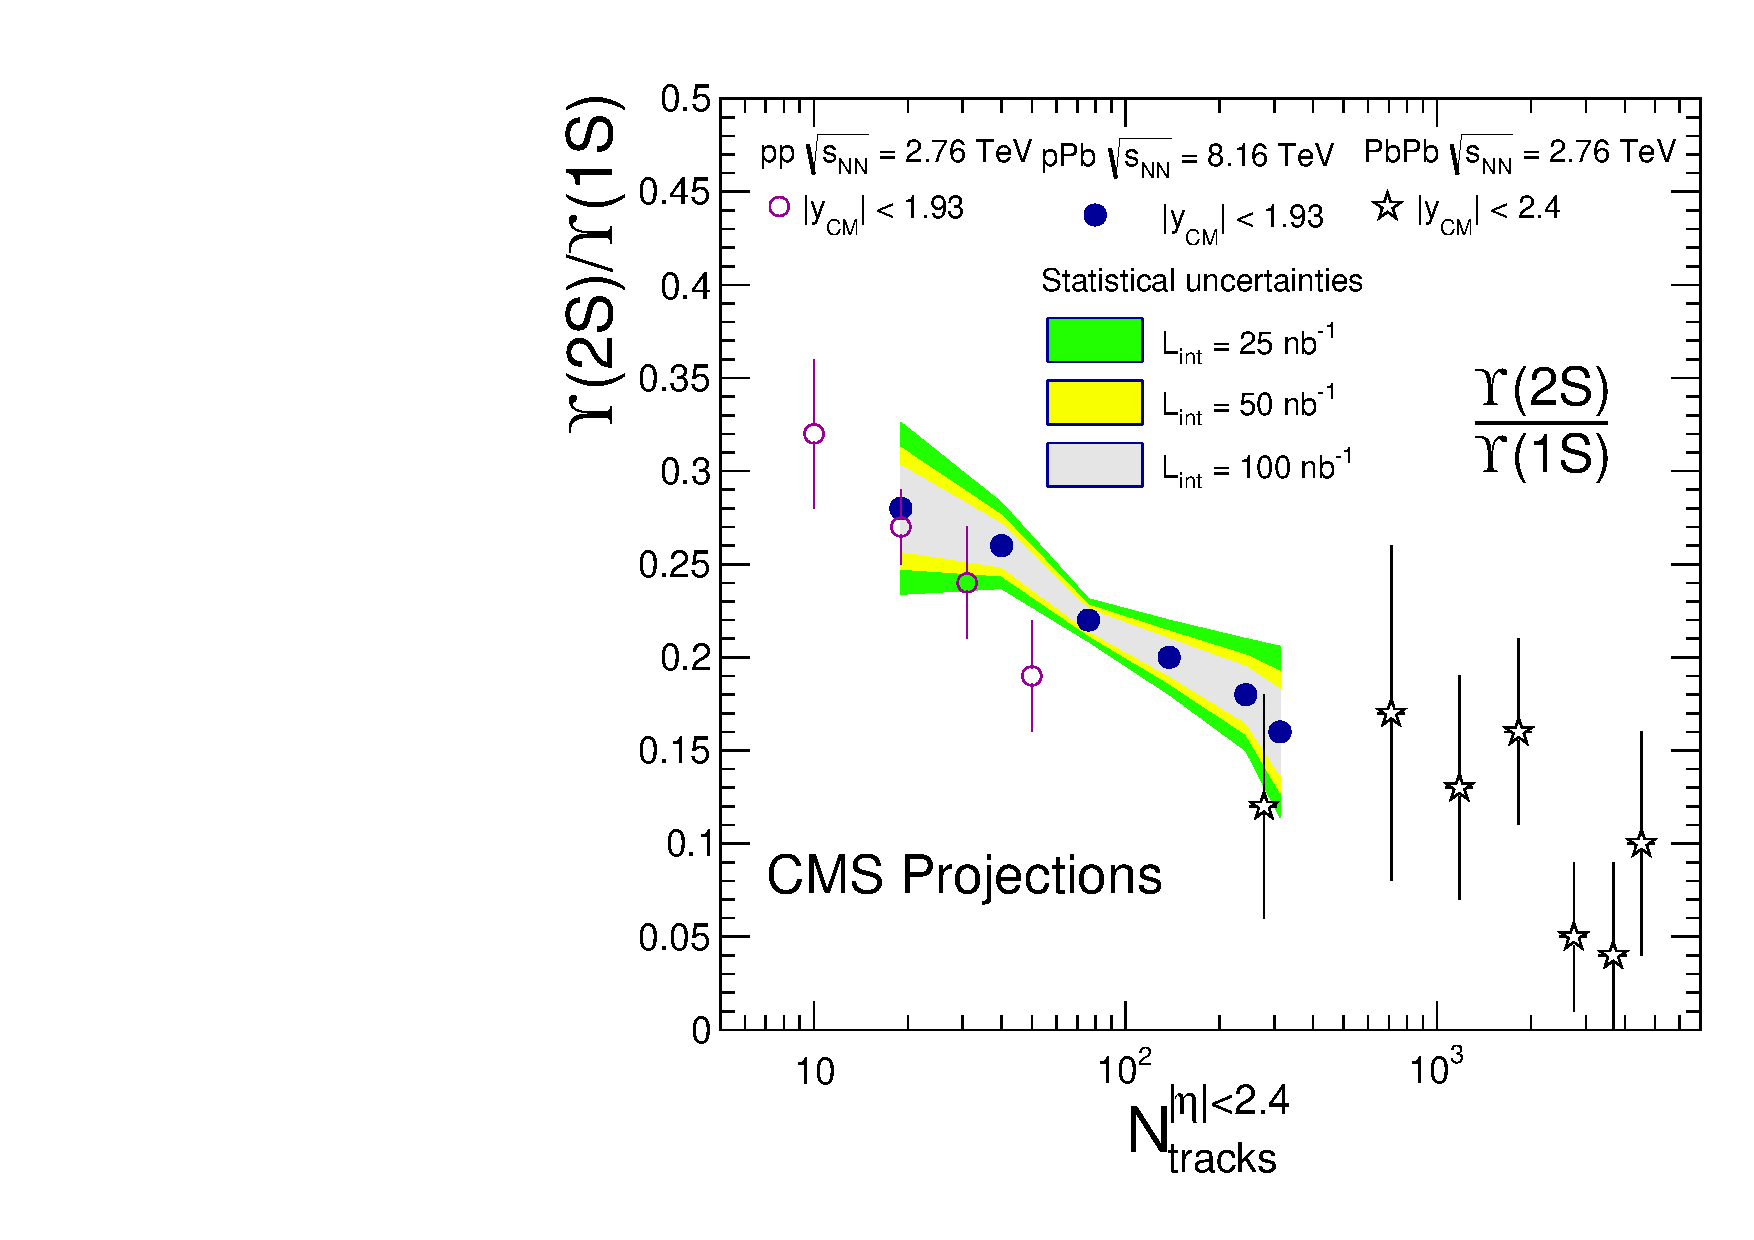
\includegraphics[width=0.6\textwidth]{figures/Upsilon_pPb_proj_combineLumi.pdf}
    \caption{ 
    }
    \label{fig:UpsilonvsNtrk}
  \end{center}
\end{figure} 

\begin{figure}[thb]
  \begin{center}
    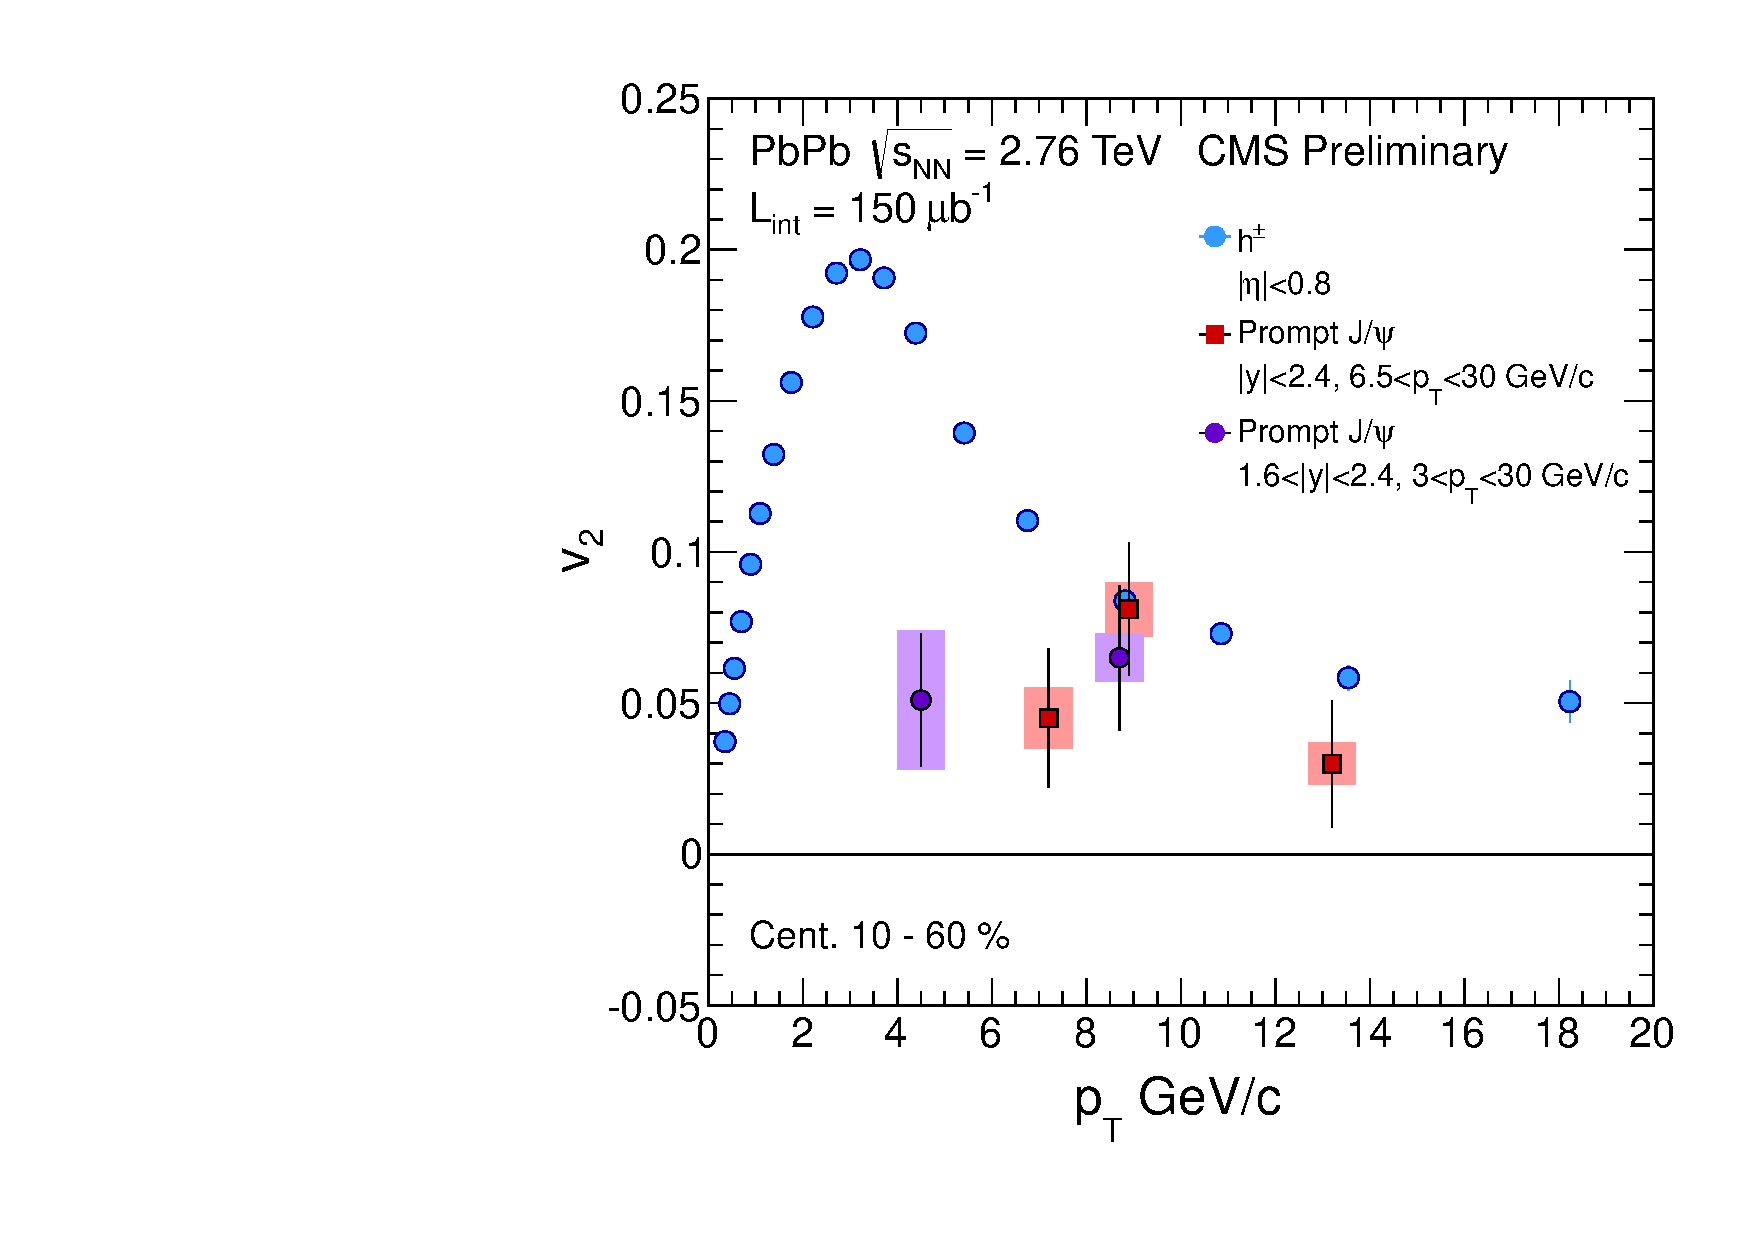
\includegraphics[width=0.6\textwidth]{figures/comp_v2_pTs_CMSflow_Prp_Cor.pdf}
    \caption{ 
    }
    \label{fig:v2_Jpsi}
  \end{center}
\end{figure} 

\clearpage
\section{Nuclear PDF}

\subsection{Dijets of light and heavy flavors}


\begin{figure}[h]
\begin{center}
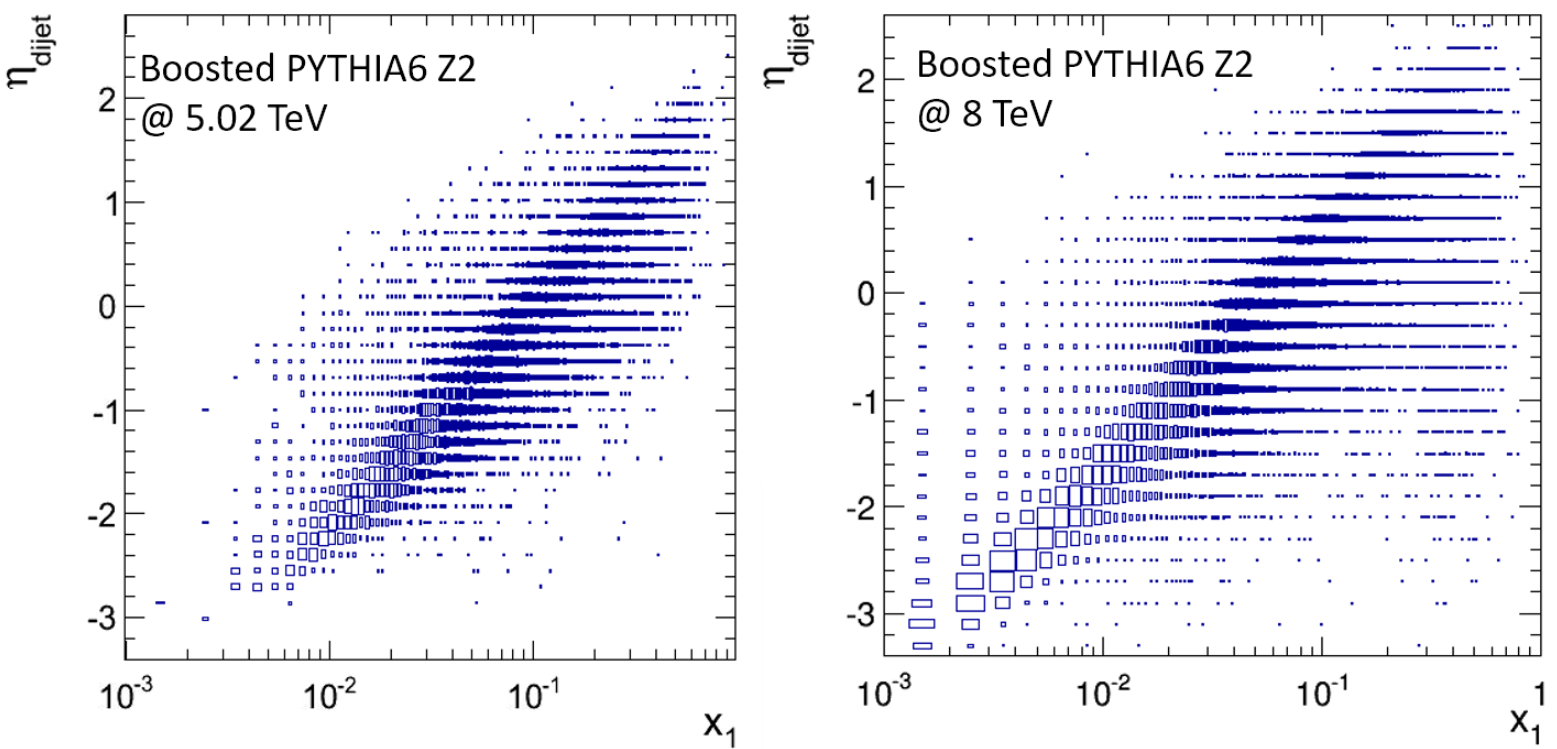
\includegraphics[width= 0.9\textwidth]{figures/x_vs_eta.png}
\caption{Correlations between dijet $\eta_{\rm dijet} = \eta_{1} + \eta_{2}$ 
and parton Bjorken-$x$ from Pb nuclei at \rootsNN\ = 5.02 TeV 
(left) and 8.16 TeV (right) from the boosted {\sc pythia} event generator.}
\label{fig:dijetCorr}
\end{center}
\end{figure}

The measurement of dijet pseudorapidity distributions were 
shown to be sensitive to nPDF effects~\cite{Paukkunen:2014pha}.
Earlier CMS measurement in pPb collisions at \rootsNN\ = 5.02 TeV
has been used to discriminate between different nPDF sets~\cite{Chatrchyan:2014hqa}. 
The tight correlation shown in Fig.~\ref{fig:dijetCorr} between 
dijet $\eta_{\rm dijet} = \eta_{1} + \eta_{2}$ and parton $x$ from Pb nuclei
is the underlying reason of the sensitivity to nPDF. At \rootsNN\ = 8.16 TeV, 
the slope of the correlation varies as $x \approx 1/\sqrt{s_{\rm NN}}$. 
This allows us to push toward a wider $x$ coverage at higher collision energy
within the same detector acceptance. Moreover, with the increase in 
di-b-jet cross section at \rootsNN\ = 8.16 TeV. It will be possible to perform 
the measurement of $\eta_{\rm dijet}$ distributions where both 
leading and subleading jets are tagged as b-jets. As 96\% of 
di-b-jet production is from gluon fusion processes, such a measurement
will be a clean probe of gluon nPDF.


\begin{figure}[h]
\begin{center}
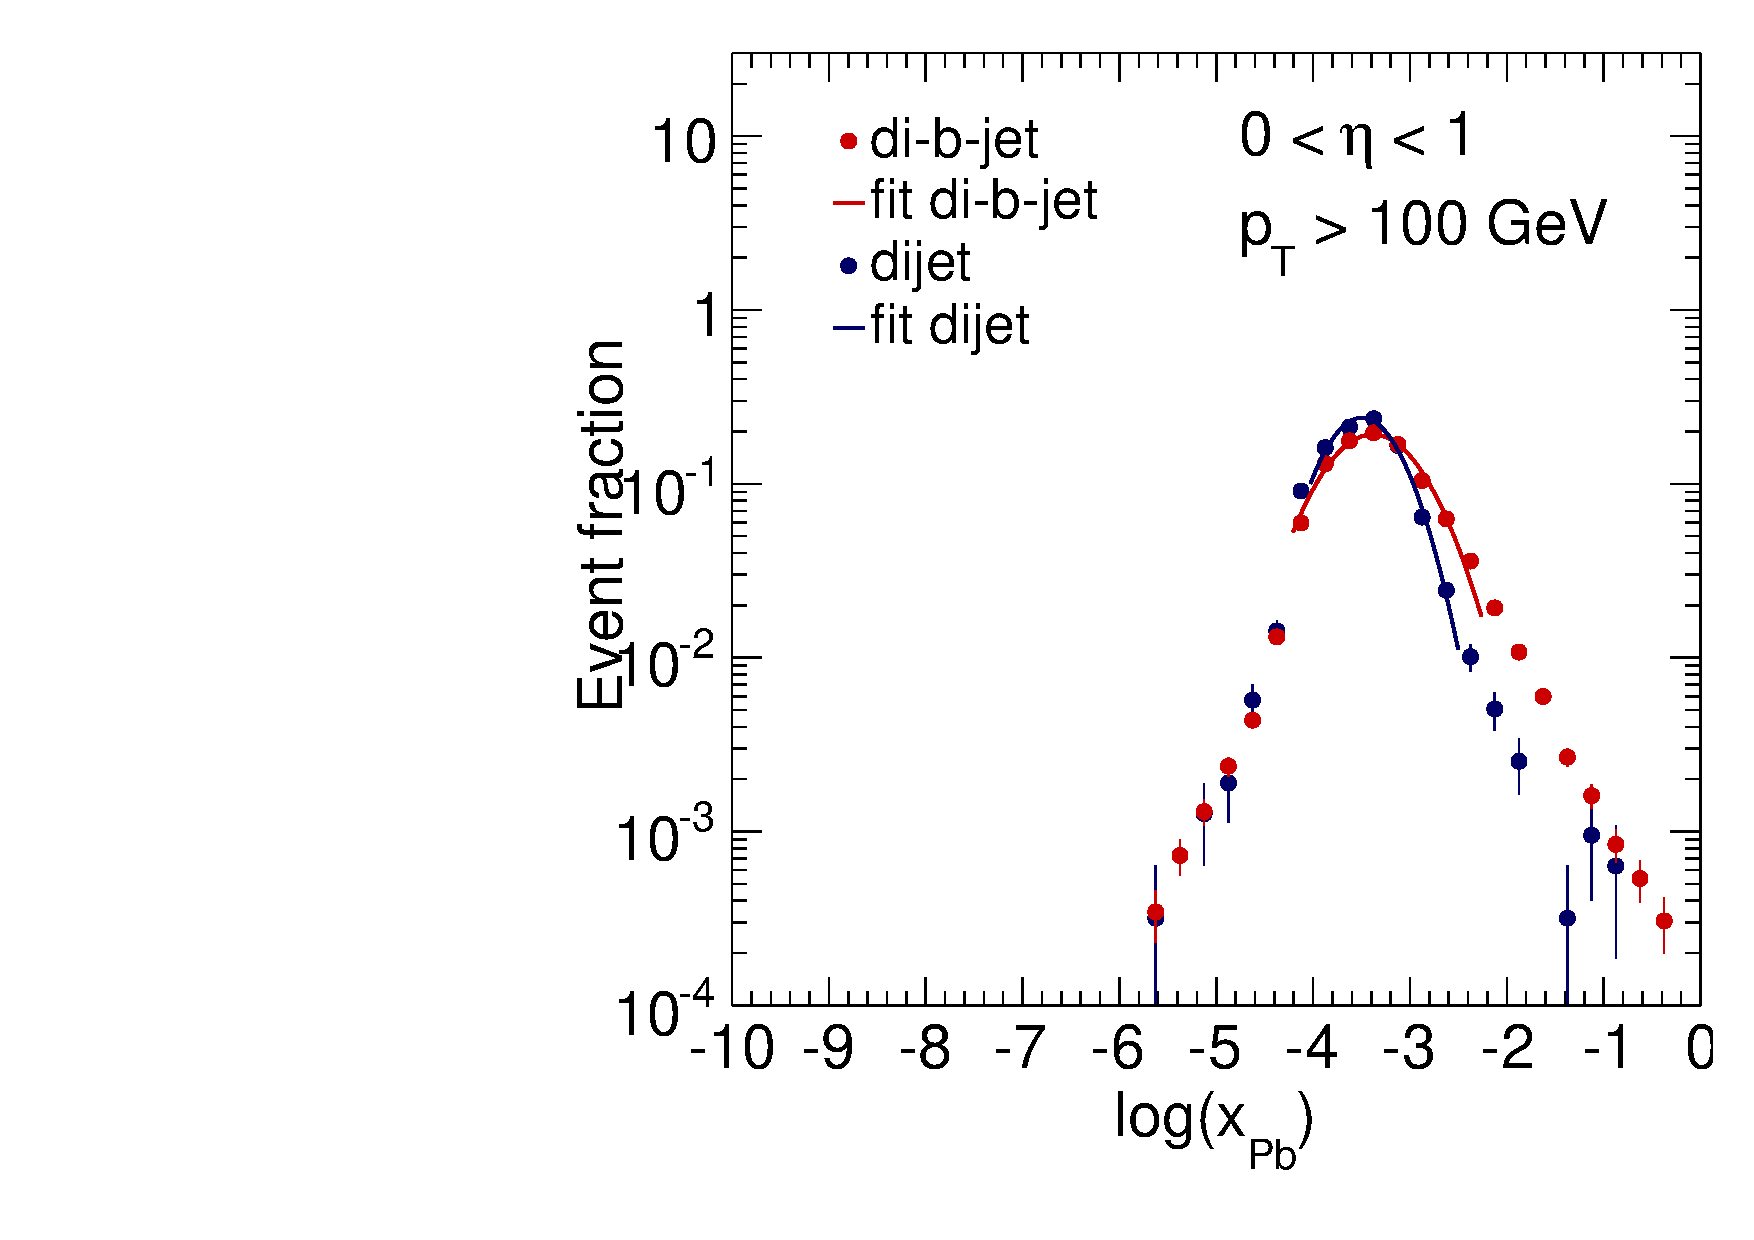
\includegraphics[width= 0.4\textwidth]{figures/DistCompareBJetInclusive.pdf}
\caption{ Distribution of $x_{\rm Pb}$ in log scale for $0<\eta_{\rm dijet}<1$
and $\pt^{\rm ave} > 100$ GeV/c in boosted {\sc pythia} event generator.}
\label{fig:distX}
\end{center}
\end{figure}

Different $x$ values can be probed by selecting on $\eta_{\rm dijet}$, 
while different $Q$ values can be chosen by posing requirements 
on the average \pt\ of the dijets $\pt^{\rm ave} = (p_{\rm T,1} + p_{\rm T,2})/2$.
The expected $x$--$Q$ coverage is calculated by parametrizing 
the $x_{\rm Pb}$ distributions in boosted {\sc pythia} event generator
for a specific $\eta_{\rm dijet}$ and $\pt^{\rm ave}$ selections. 
An example case is shown in Fig.~\ref{fig:distX}. To get a cleaner
estimate of dijet contributions, Gaussian fits are performed 
to exclude the long tails on both sides of the distribution, which are 
potentially contaminated by 3-jet events. The region of the Gaussian
curves outside a certain winder around the mean is scaled
according to the expected integrated luminosity. The region of sensitivity is determined 
by when the number of events outside of this region on either side of 
the mean, given as $0.5 \times {\rm ErfcInverse}((x-\mu)/(\sqrt{2}\sigma))$, 
falls below $1/\epsilon_{\rm stat}^{2}$. The same procedure is also applied 
in deriving the sensitive region of $Q$. The reach in $x$ and $Q$ values 
are calculated in several bins of $\eta_{\rm dijet}$ and $\pt^{\rm ave}$ 
and overlaid as patches of areas on the $x$--$Q$ plane. The results are shown 
in Figs.~\ref{fig:xQscanBjet} for di-b-jets and \ref{fig:xQscanInclusive} 
for inclusive dijets, respectively.


\begin{figure}[h]
\begin{center}
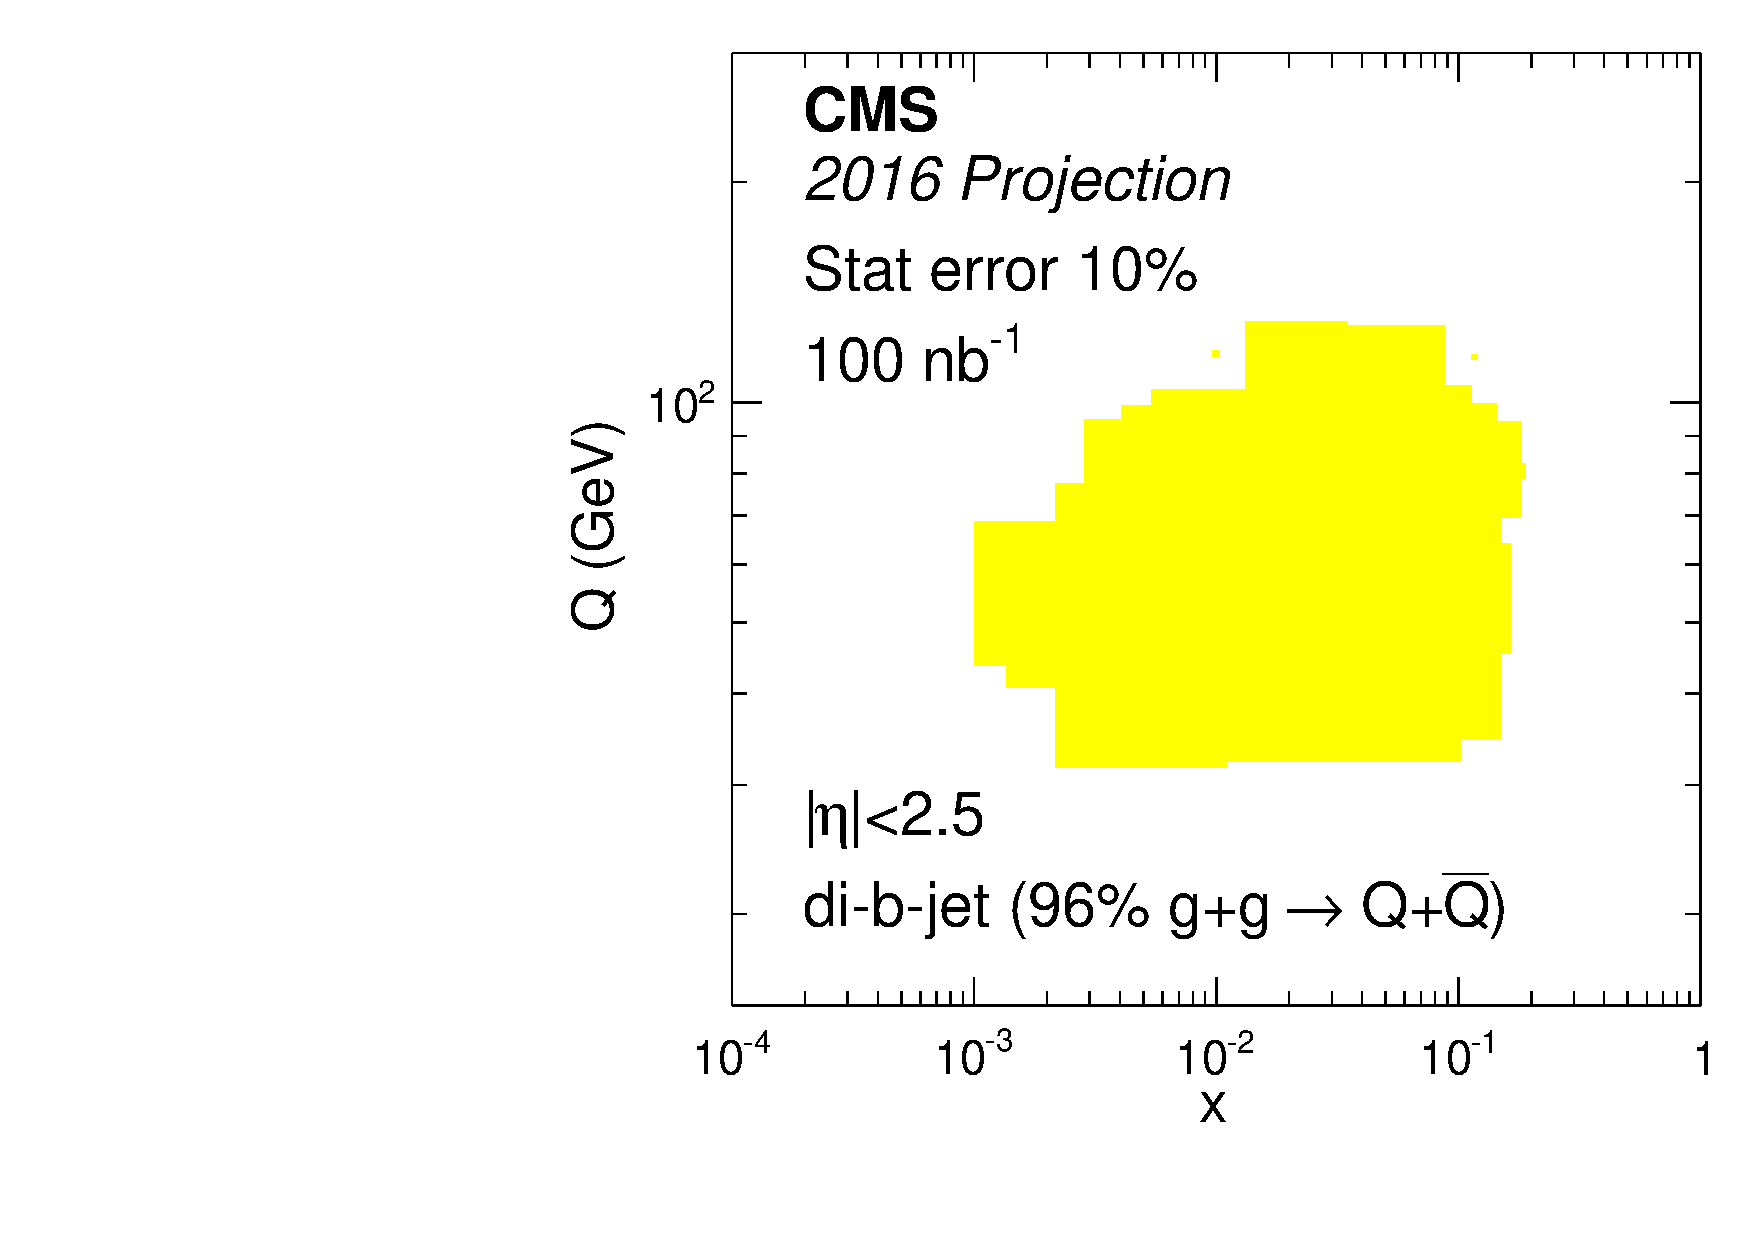
\includegraphics[width= 0.47\textwidth]{figures/filledQX_Lumi100_BJet.pdf}
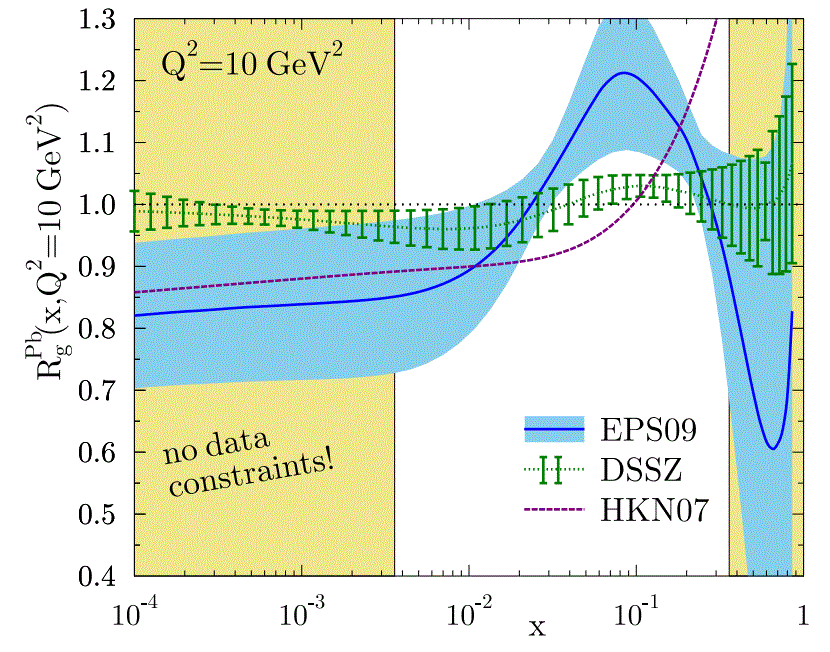
\includegraphics[width= 0.47\textwidth]{figures/eps09_10GeV_Gluon_nPDF.png}
\caption{Left: The $x$--$Q$ scan plot for di-b-jet processes 
with an integrated luminosity of 100 nb$^{-1}$ for pPb collisions
at \rootsNN\ = 8.16 TeV. Right: The gluon nuclear modification factors 
for the lead nucleus at $Q^{2}$ = 10 GeV$^{2}$.}
\label{fig:xQscanBjet}
\end{center}
\end{figure}

Assuming an integrated luminosity of 100 nb$^{-1}$ for pPb collisions
at \rootsNN\ = 8.16 TeV, the resulting $x$--$Q$ scan plot for di-b-jet processes 
is shown in Fig.~\ref{fig:xQscanBjet} (left). As one can see, a high-luminosity
pPb run in 2016 will provide constraints to nPDF in small-$x$ region down to
$3-4 \times 10^{-3}$. In this $x$ regime, there are no existing data
constraints to the gluon nPDF, as shown in Fig.~\ref{fig:xQscanBjet} (right)~\cite{Paukkunen:2014nqa}.

\begin{figure}[h]
\begin{center}
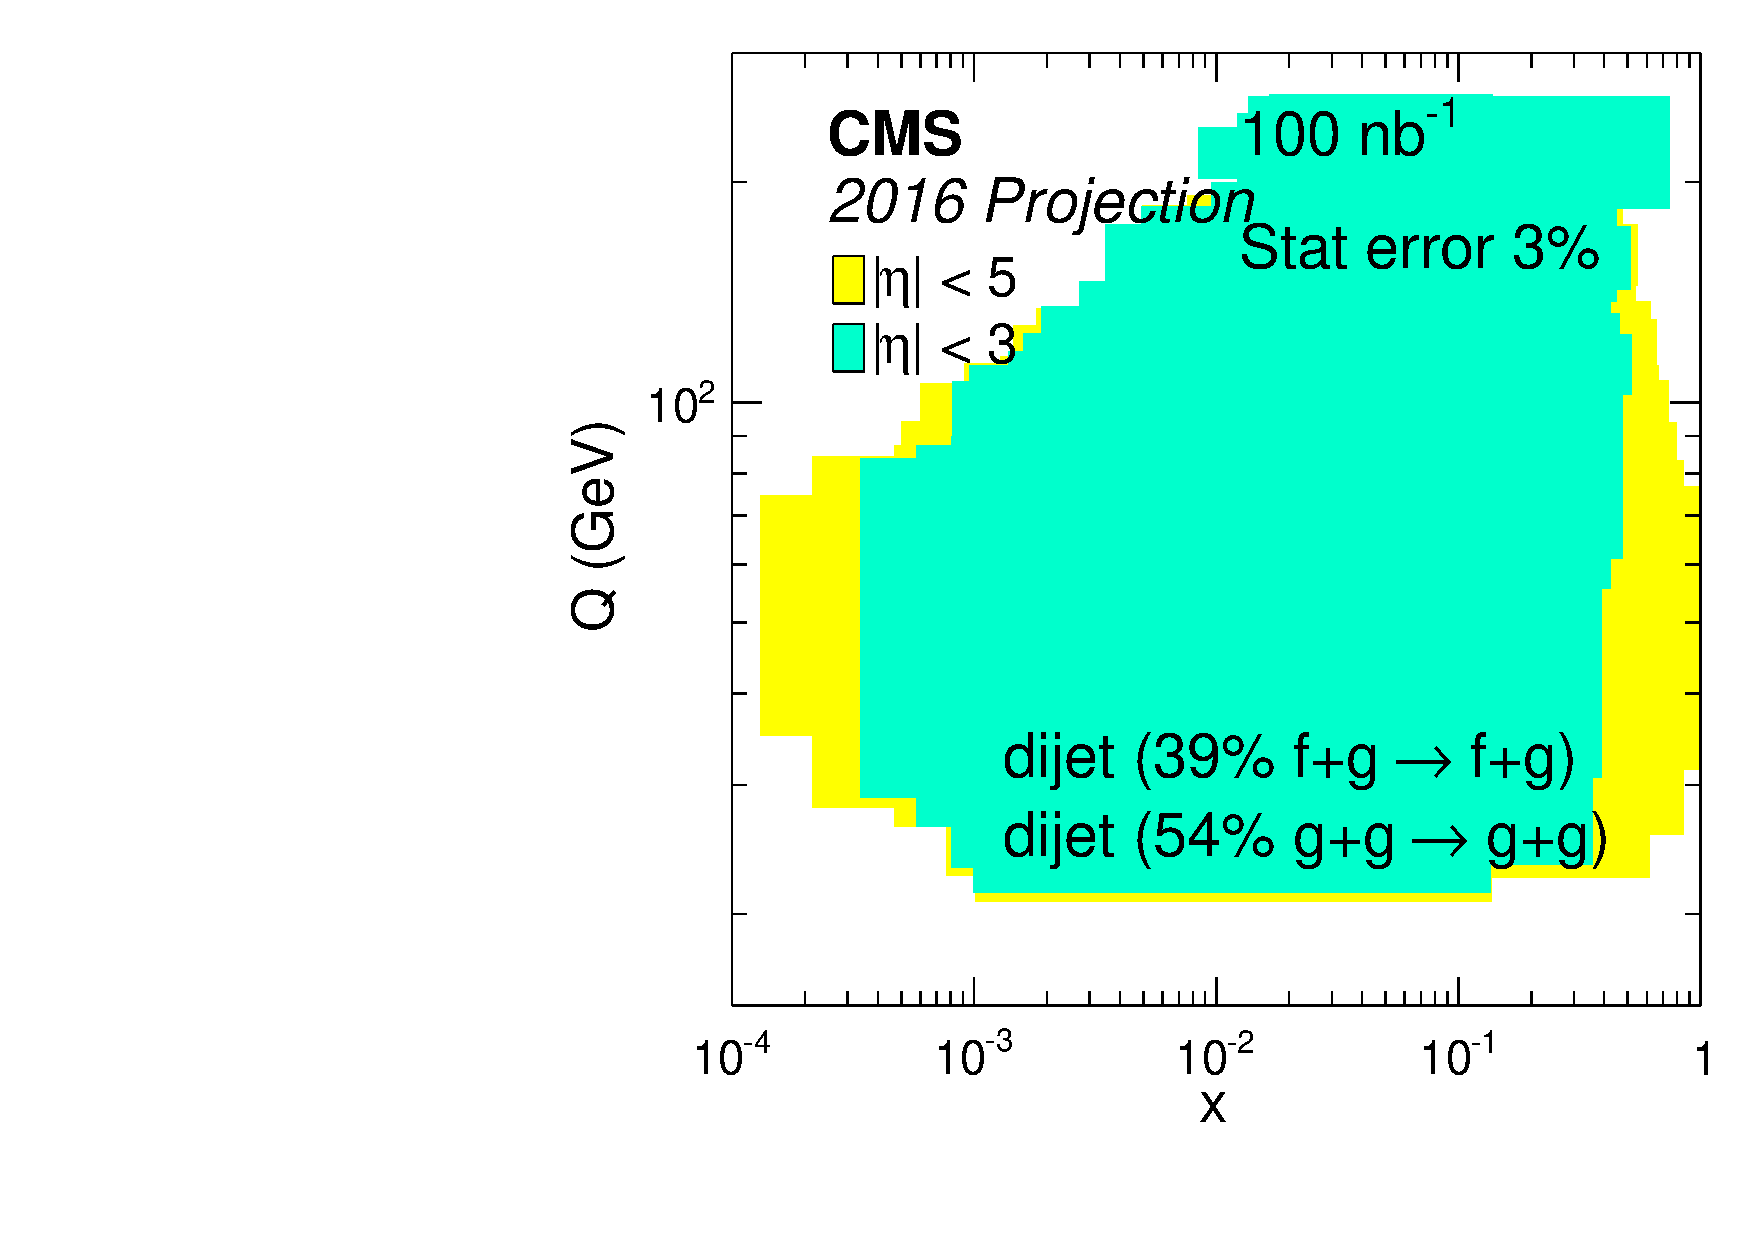
\includegraphics[width= 0.5\textwidth]{figures/filledQX_Lumi100_InclusiveJet_etaComparison.pdf}
\caption{The $x$--$Q$ span of inclusive dijet measurement for the two pseudorapidity selections 
for a measurement with better than $3\%$ statistical precision. }
\label{fig:xQscanInclusive}
\end{center}
\end{figure}


For inclusive flavor dijets, there are significant contributions
from $f + g \rightarrow f + g$ ($39 \%$) processes in addition to gluon fusion 
($54 \%$) processes.Therefore, they do not provide a clean handle on 
the gluon nPDF, which is much less constrained comparing to quark nPDF.
However, due to an abundance of inclusive dijets produced in the collisions,
they can be used to probe a much wider $x$--$Q$ range. The $x$ reach of b-jet measurement 
is limited by the $\eta$ coverage of the tracker, i.e. $|\eta| < 2.5$. 
However, the untagged flavor jet measurements can be extended up to 
$\eta = 3$ with good control on systematic uncertainties and up to $\eta = 5$ if the total 
integrated luminosity is sufficient to allow one to calibrate the energy response of 
Hadronic Forward (HF) calorimeters. The $x$--$Q$ span of inclusive dijet 
measurement is shown in Fig.~\ref{fig:xQscanInclusive} for the two pseudorapidity selections 
for a measurement with better than $3\%$ statistical precision. 
The statistical uncertainty as a function of $x$ in the high-$x$ region 
is shown in Fig.~\ref{fig:XreachWithPseudorapidity} for different 
luminosity scenarios, 10, 25, 50 and 100 nb$^{-1}$, for $|\eta| < 3$ (left) 
and for $|\eta| < 5$ (right). For dijets selected 
within $|\eta| < 3$, where systematic uncertainties are well under control, 
the reach in large-$x$ regime clearly benefits from a high-luminosity pPb run. 
With an integrated luminosity of 100 nb$^{-1}$, it is possible to measure up to $x = 0.6$ 
within $10 \%$ statistical accuracy.

\begin{figure}[h]
\begin{center}
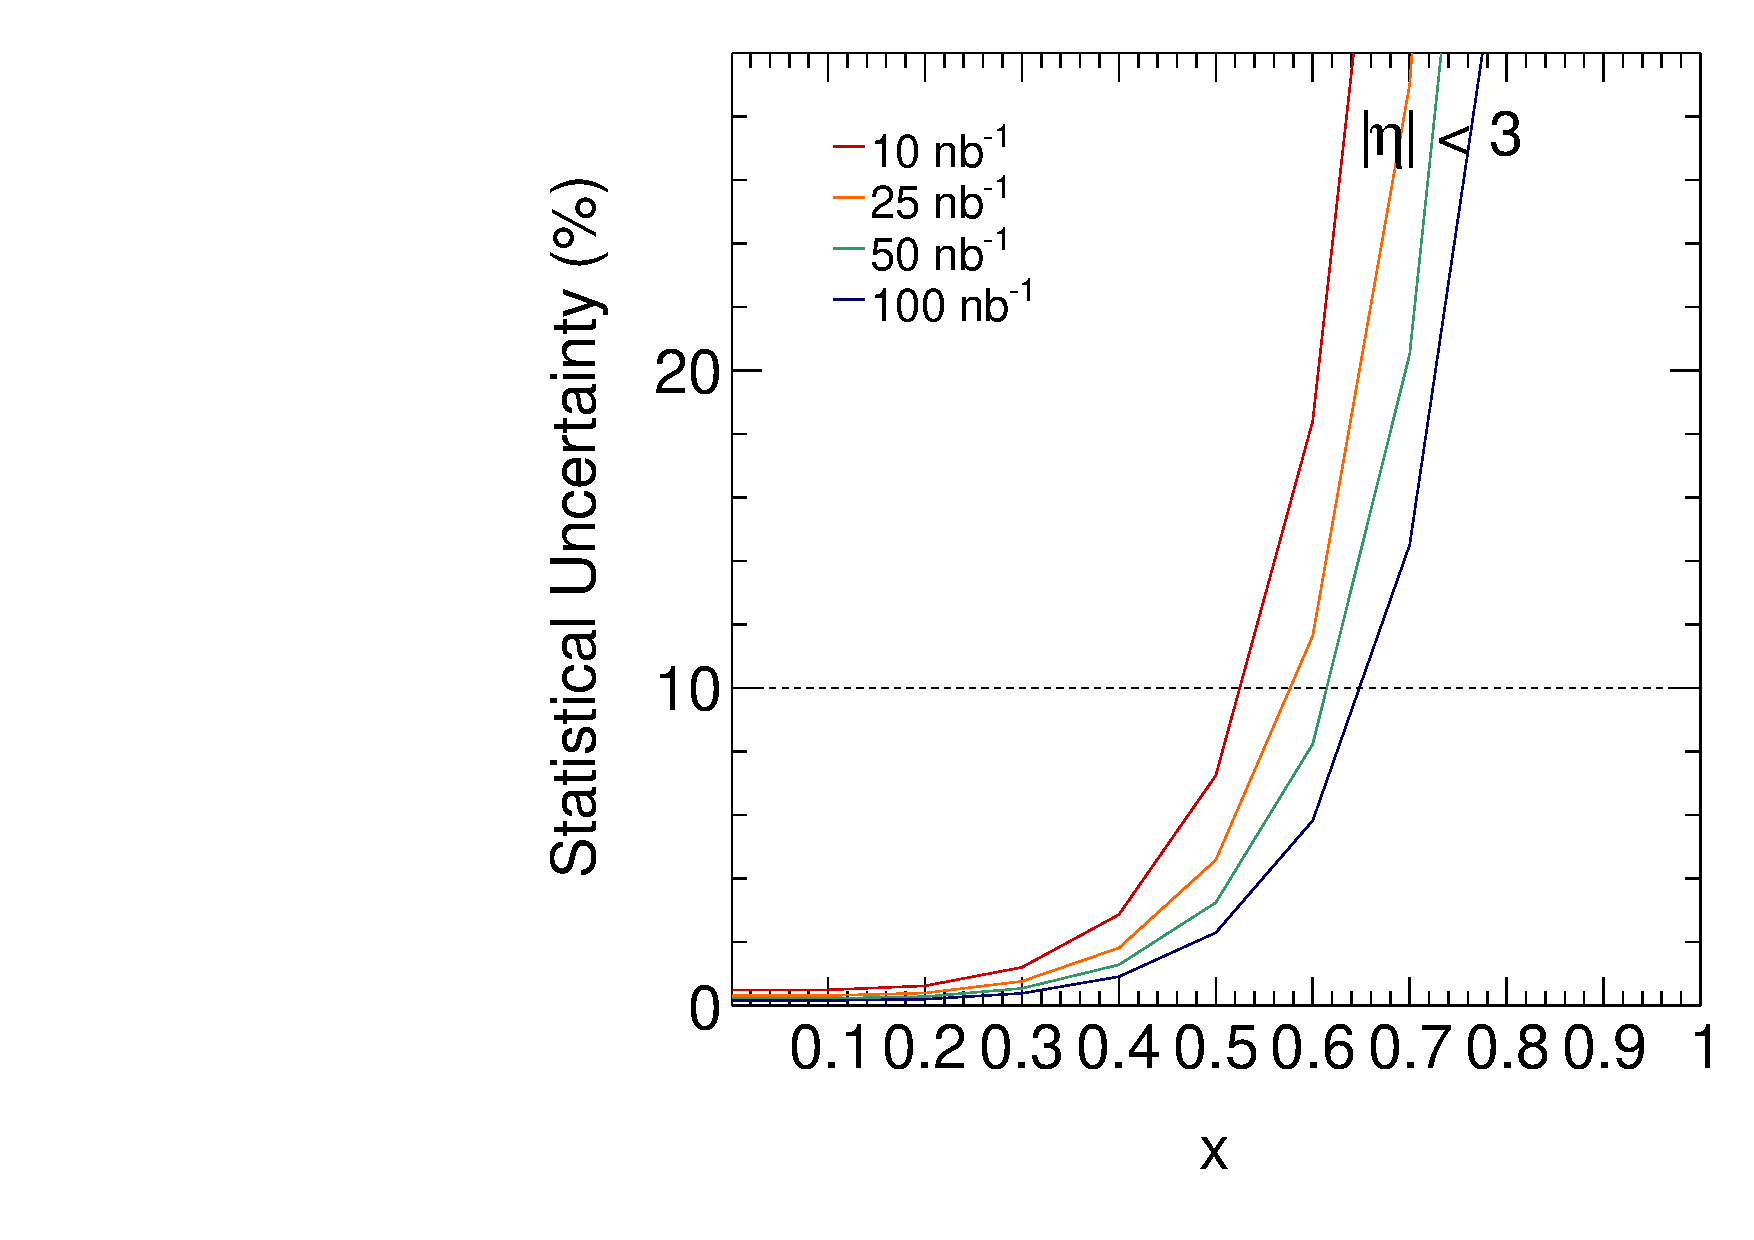
\includegraphics[width= 0.4\textwidth]{figures/xStat_eta3_inclusiveJet.pdf}
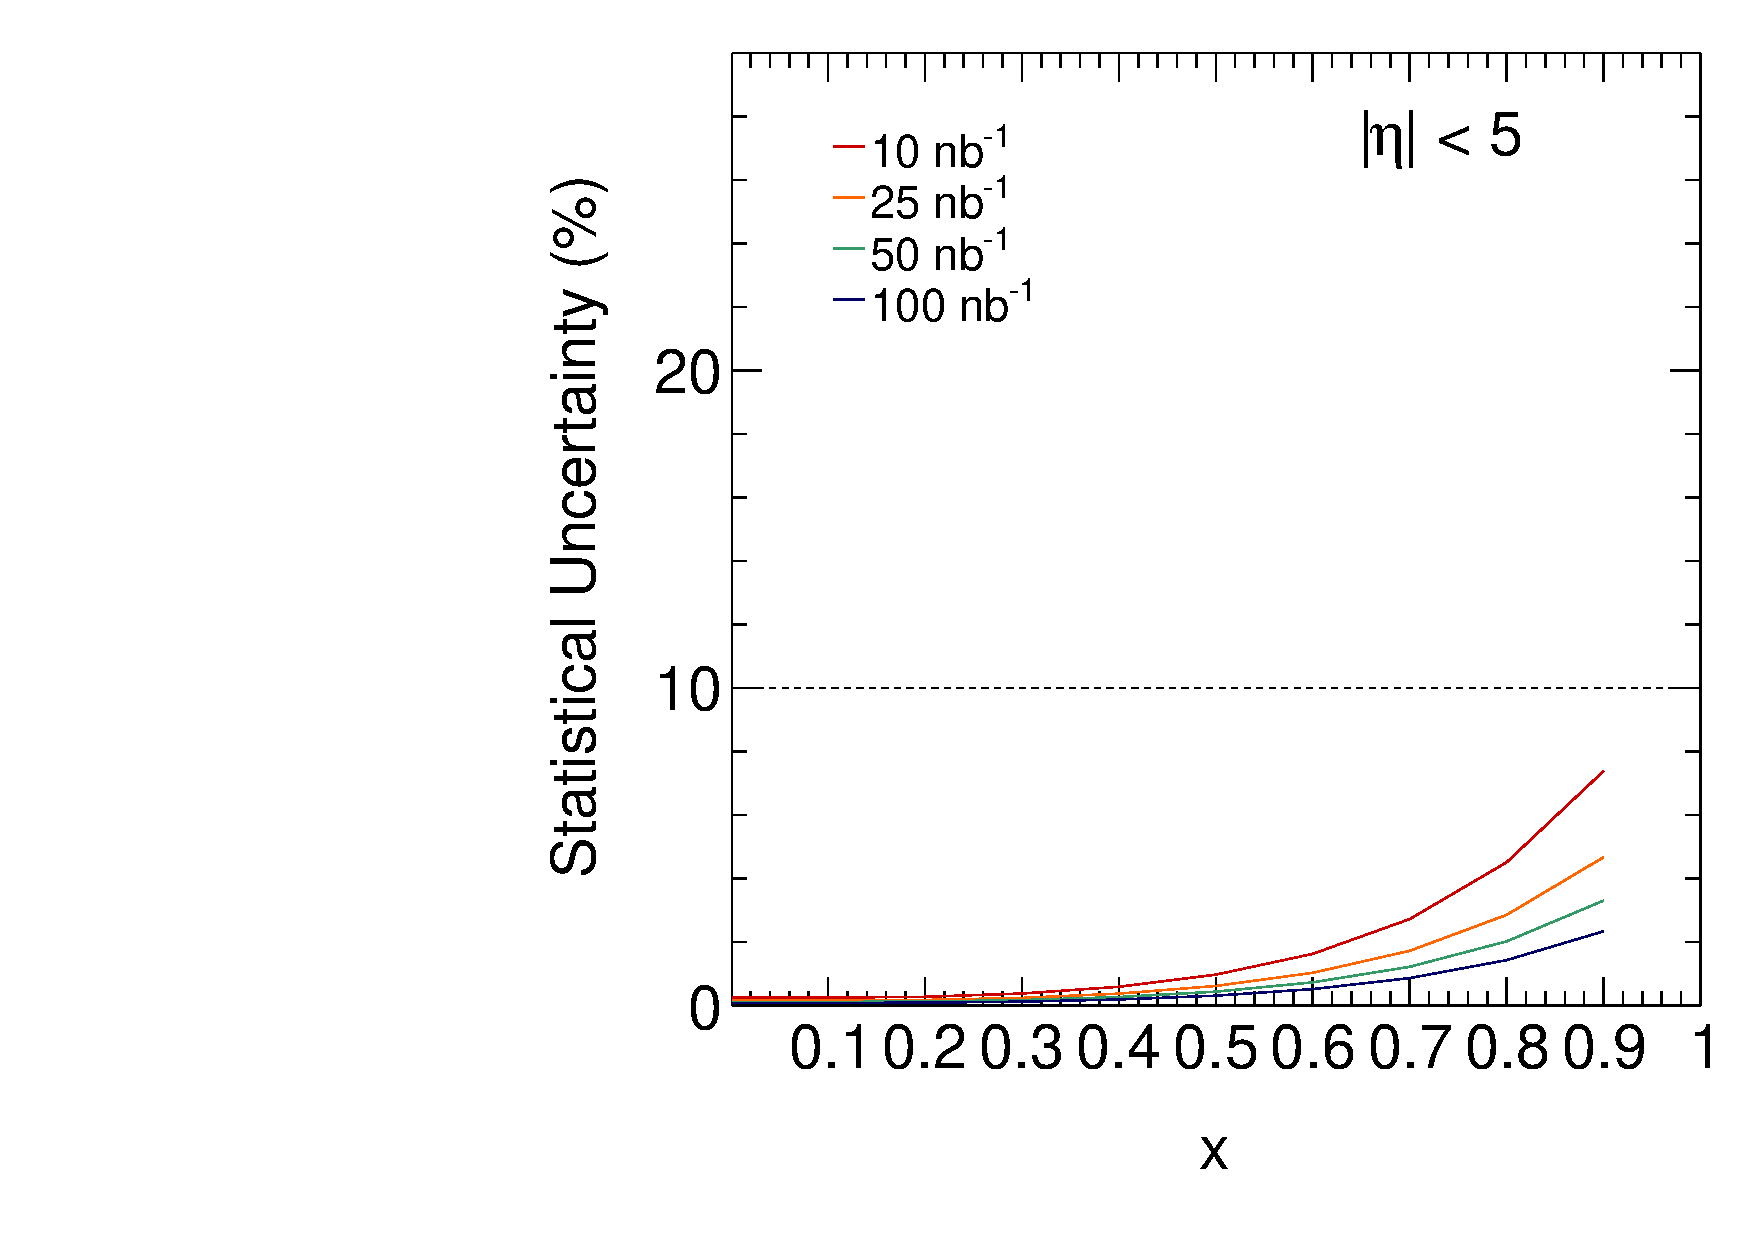
\includegraphics[width= 0.4\textwidth]{figures/xStat_eta5_inclusiveJet.pdf}
\caption{The projected statistical uncertainty as a function of $x$ in the high-$x$ region 
for different luminosity scenarios of L$_{\rm int}$ = 10, 25, 50 and 100 nb$^{-1}$, 
for $|\eta| < 3$ (left) and for $|\eta| < 5$ (right).}
\label{fig:XreachWithPseudorapidity}
\end{center}
\end{figure}

For $|\eta| < 5$ selection, the statistical uncertainty becomes negligible
and is no longer the dominant factor on the precision of the measurement. 
Systematic uncertainties caused by the jet energy scale uncertainties in HF 
become more significant. With increased integrated luminosity, the systematic 
uncertainties can also be reduced by applying data-driven methods to calibrate HF.
This has been demonstrated in pp data at \roots\ = 7 and 8 TeV, as shown in 
Fig.~\ref{fig:jetJES}. Even with L$_{\rm int}$ = $36$ pb$^{-1}$ pp data sample, 
the uncertainty on corrections in HF is $\approx 10 \%$. These uncertainties shrink 
to only $4\%$ with an integrated luminosity of $20$ fb$^{-1}$. Therefore, it will 
only be possible to probe high-$x$ values that are sensitive to a very 
interesting range of nPDF modifications with high luminosity data.

\begin{figure}[h]
\begin{center}
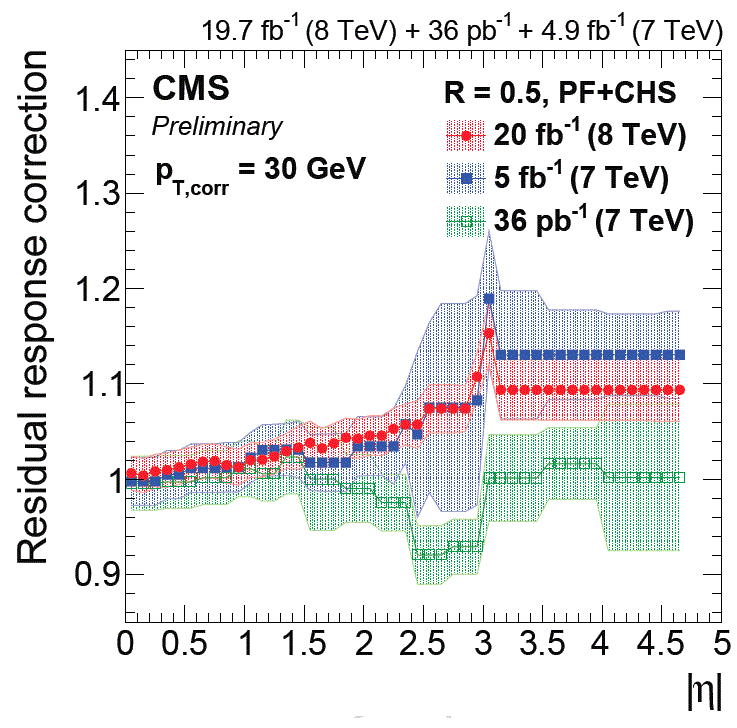
\includegraphics[width= 0.45\textwidth]{figures/staterror_jec_luminosity_pp.png}
\caption{Residual jet energy scale correction and its uncertainty as a function of
$\eta$ derived from different pp data sets at \roots\ = 7 and 8 TeV.}
\label{fig:jetJES}
\end{center}
\end{figure}

\clearpage
\subsection{D and B mesons}
A high statistics sample of pPb collisions will be extremely useful to test heavy-flavour production over a wide transverse momentum range.
At low $\rm p_{T}$, the study of the nuclear modification factors of D and B mesons allows to test the relevance of cold nuclear matter effects in the 
heavy flavour sector~\cite{Eskola:2009uj,deFlorian:2003qf,Frankfurt:2011cs}. Gluon saturation processes are expected to reduce the production 
cross sections of D mesons of about 10-20$\%$ at about 2-3 GeV/c.  
In the B sector, a smaller modification is expected as a consequence of the large $x$ range that we investigate with this measurement.
A precise measurement of the D and B nuclear modification factors in pPb collisions at low $\rm p_{T}$ is therefore needed to experimentally validate
the theoretical expectations.
In Fig~\ref{fig:measurementB}, the current measurement performed at 5.02 TeV with  $\rm L_{int}$=34.8/nb is presented~\cite{PhysRevLett.116.032301}. The current statistical 
and systematic uncertanties do not allow to appreciate any significant deviation from unity. In Fig~\ref{fig:Bextrapolated}, the result expected at 8 TeV
considering an integrated luminosity of 100/nb is presented. In order to have the possibility to measure the B production down to low $\rm p_{T}$ with the needed accuracy (~5-10$\%$), 
the largest luminosity available is therefore strictly necessary.  A larger sample of 8 TeV pPb data would also be beneficial for heavy flavour studies at high $\rm p_{T}$.  In Fig~\ref{fig:plotsDBpredictions}, 
the FONLL predictions for D (left) and B (right) cross sections are shown. A  increase of the heavy-flavour cross section of about 2 is
expected at $\rm p_{T}~$100 GeV/c as a consequence of the larger centre-of-mass value. 

\begin{figure}[h]
\begin{center}
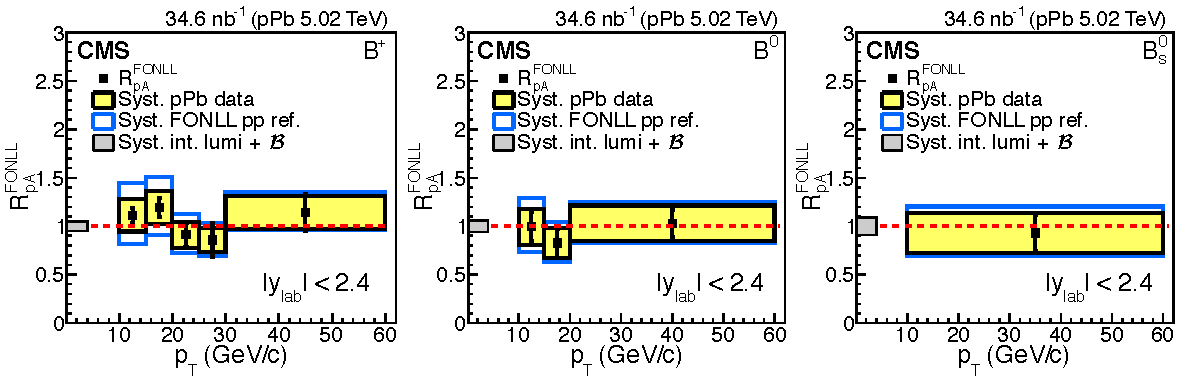
\includegraphics[width= 0.95\textwidth]{figures/nuclearmodification.pdf}
\caption{Nuclear modification factor in pPb collisions at 5.02 TeV obtained with 34.8/nb~\cite{PhysRevLett.116.032301}.}
\label{fig:measurementB}
\end{center}
\end{figure}



\begin{figure}[h]
\begin{center}
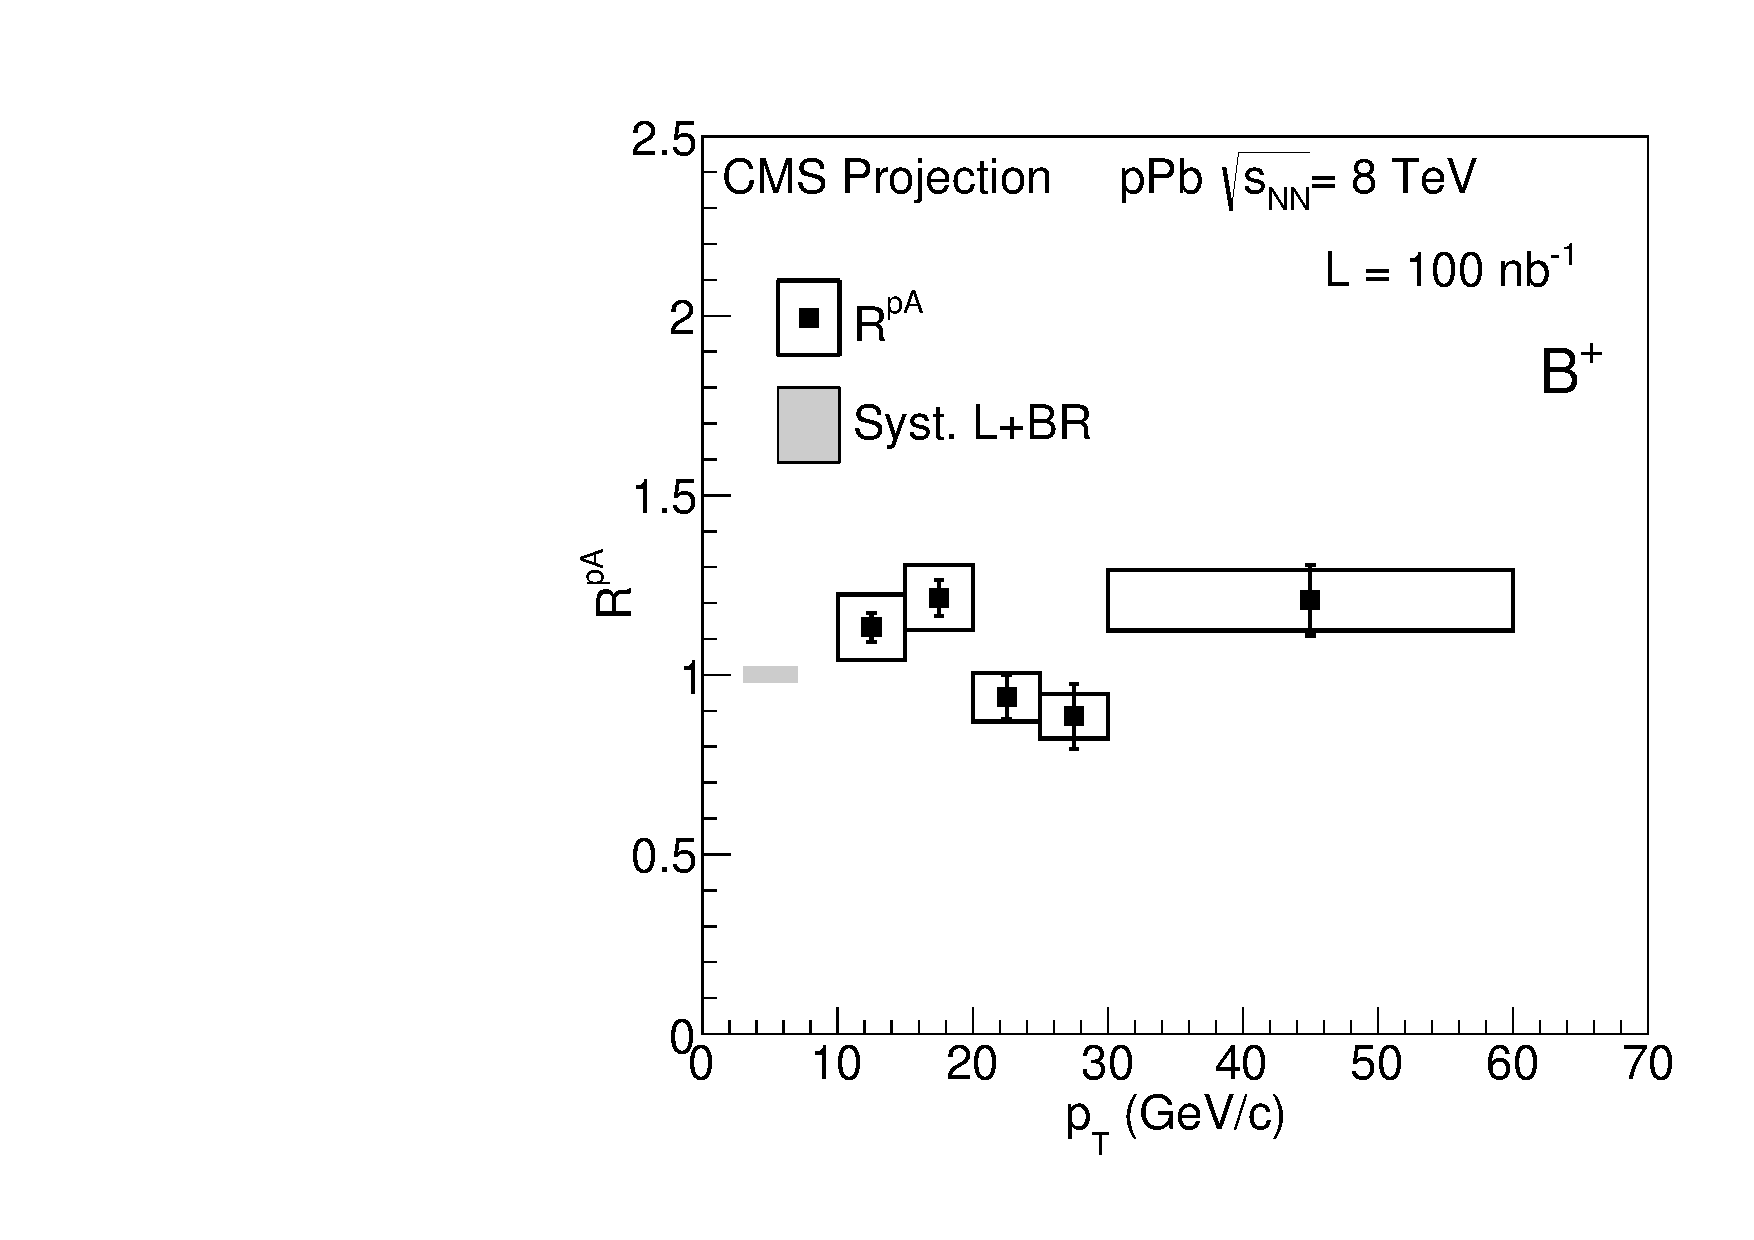
\includegraphics[width= 0.55\textwidth]{figures/canvasrpabplus}
\caption{Prediction for $\rm B^{+}$ $\rm R_{pPb}$ estimated with a luminosity of $\rm L_{int}$=100/nb based on 2011 pPb measurement.}
\label{fig:Bextrapolated}
\end{center}
\end{figure}


\begin{figure}[h]
\begin{center}
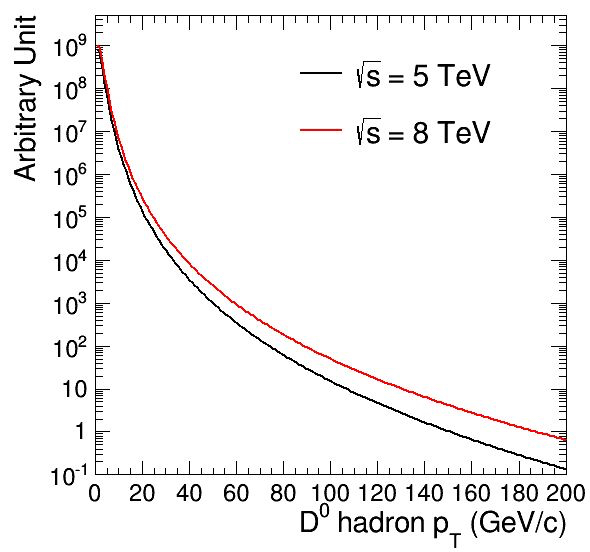
\includegraphics[width= 0.45\textwidth]{figures/D-Sigma.jpg}
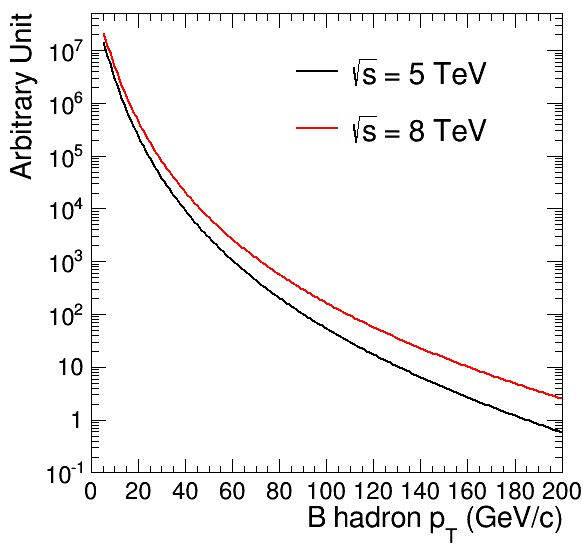
\includegraphics[width= 0.45\textwidth]{figures/B-Sigma.jpg}
\caption{FONLL predictions for D (left) and B (right) meson production at 8 and 5TeV as a function of $\rm p_{T}$~\cite{FONLLcharmbottomPP1}.}
\label{fig:plotsDBpredictions}
\end{center}
\end{figure}

\subsection{Top quarks (Marta)}
At LHC energies the dominant production channel for top pair production is gluon-gluon fusion which is responsible for 80\%-95\% of the total pair production. The remaining $\mathrm{t}\bar{\mathrm{t}}$ pairs are from quark-antiquark annihilation. 

As discussed in \cite{d'Enterria:2015jna}, top measurements probe the nuclear gluon density in an unexplored kinematic regime around Bjorken-x values, $x \sim 2m_{\mathrm{t}}/\rootsNN \sim 5 \cdot 10^{-3}-0.05$, and virtualities $Q^{2} \sim m_{\mathrm{t}}^{2} \sim 3 \cdot 10^{4}$ GeV, a region characterized by anti-shadowing corrections. 

\begin{figure}[h!]
\begin{center}
  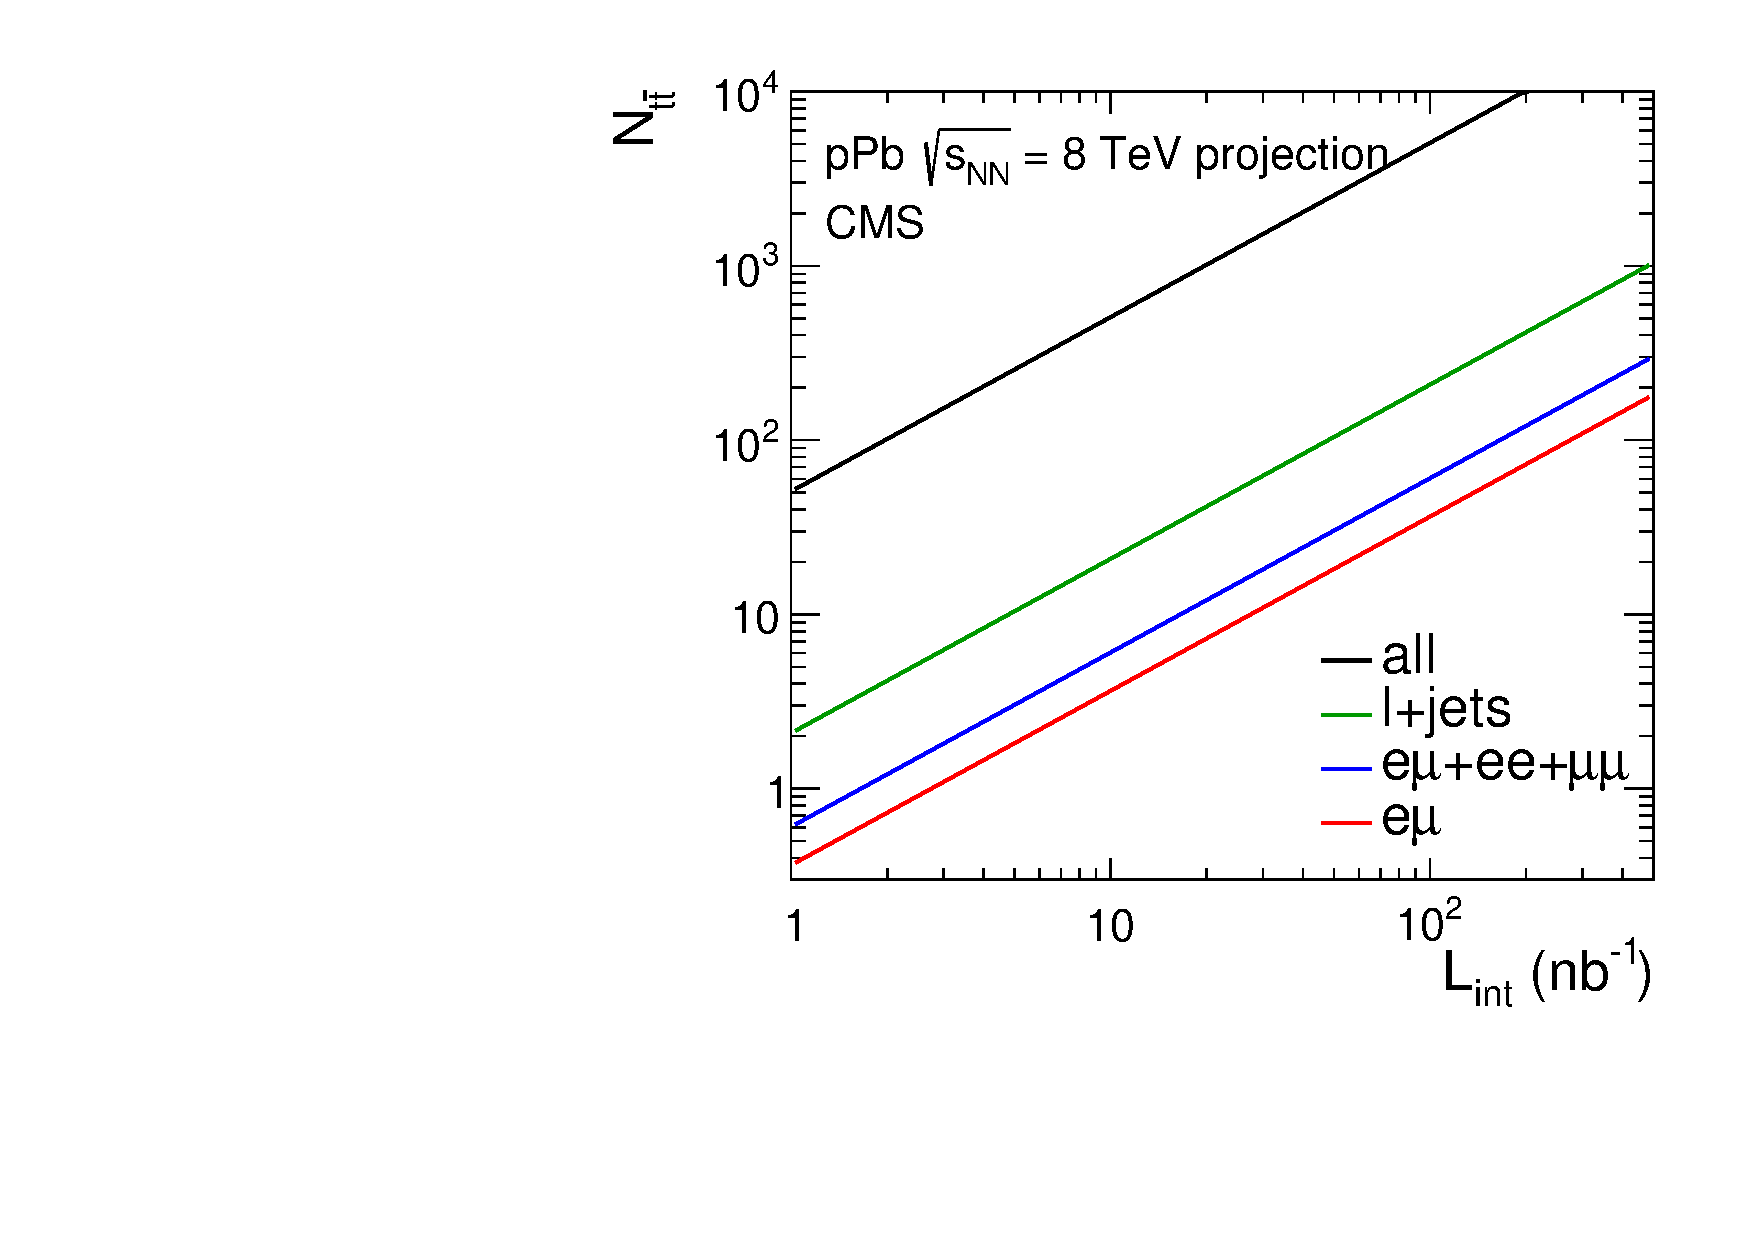
\includegraphics[width= 0.43\textwidth]{figures/top/ProjectedTTbarYield.pdf}
  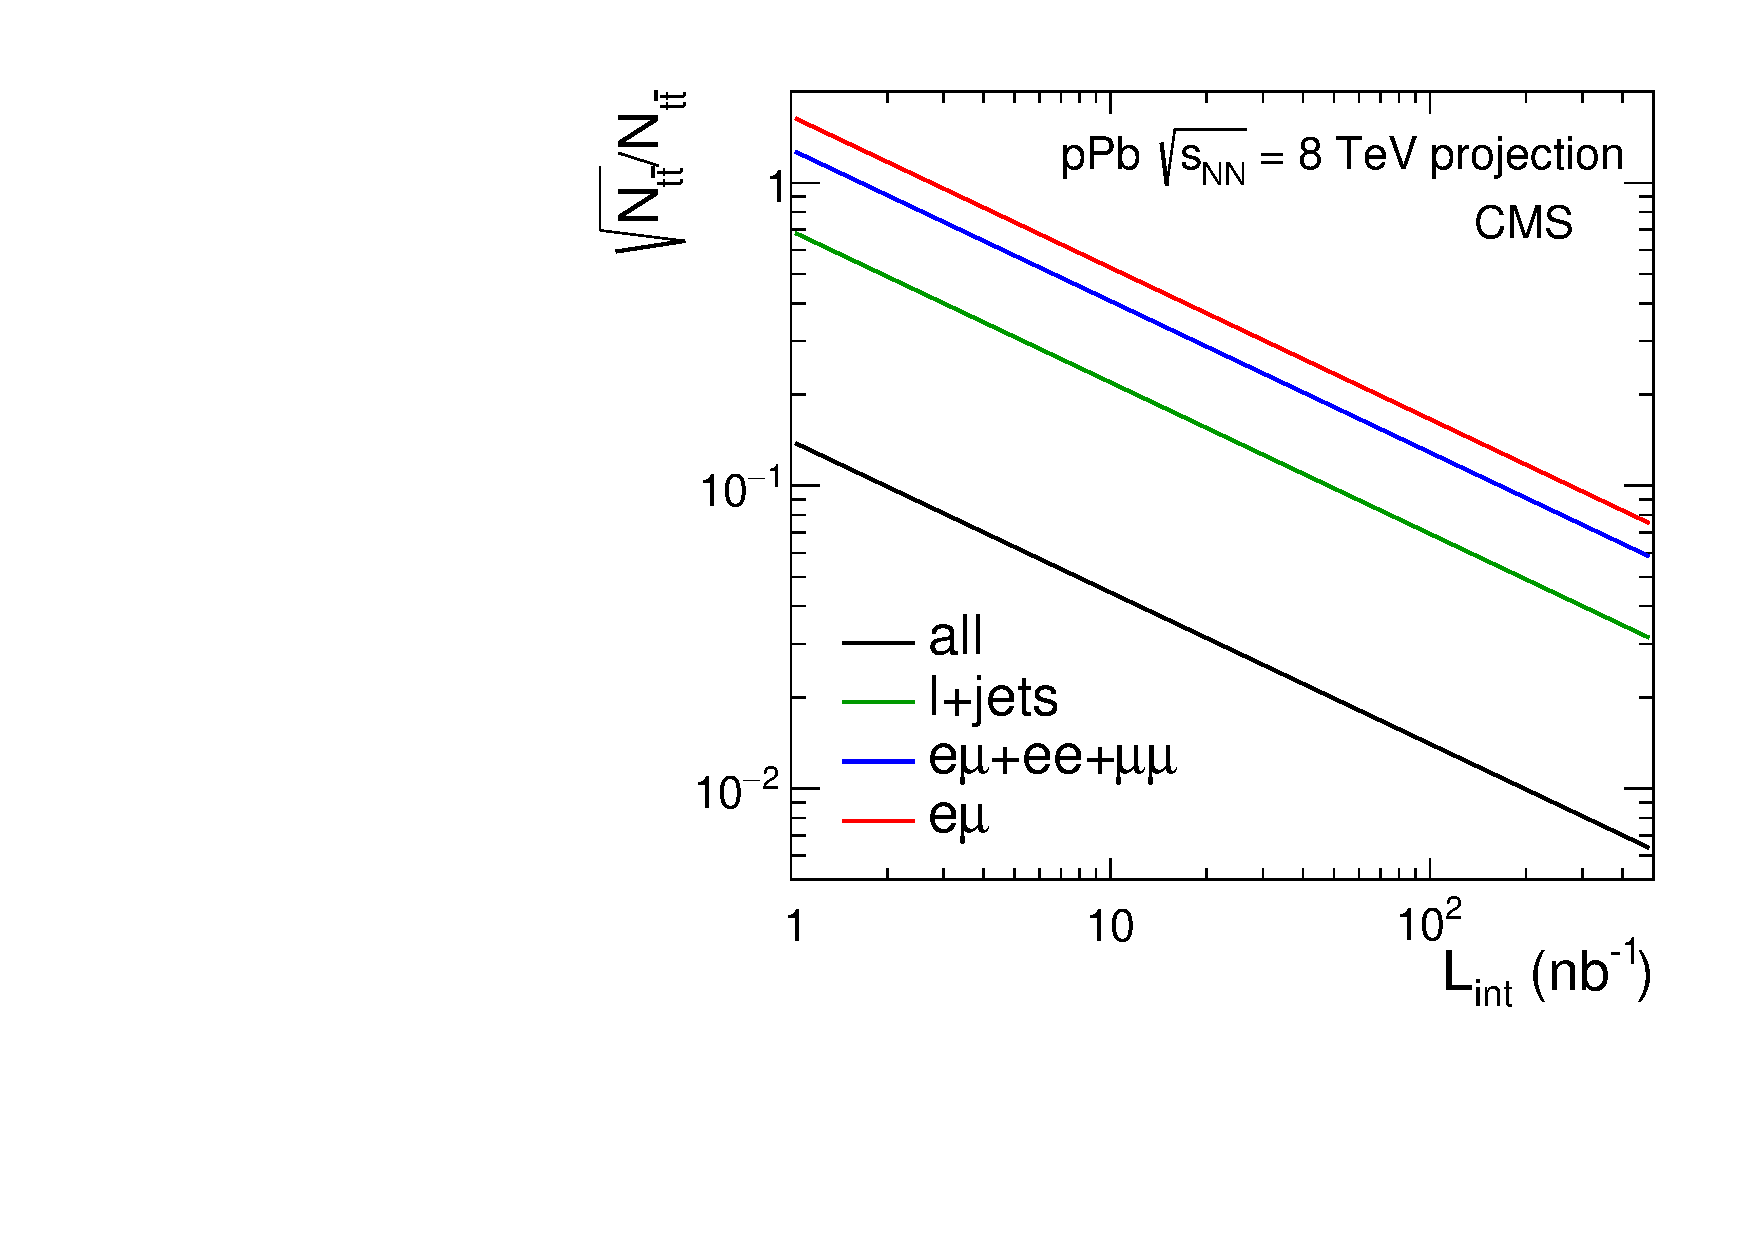
\includegraphics[width= 0.43\textwidth]{figures/top/ProjectedTTbarStatUnc.pdf}
  \caption{Left panel: Expected number of $\mathrm{t}\bar{\mathrm{t}}$ events for several channels in pPb collisions at $\sqrt{s_{\mathrm{NN}}}=8$ TeV as function of total integrated luminosity. Right panel: Corresponding statistical uncertainty as function of total integrated luminosity.
  }
\label{fig:ttPPbProjections}
\end{center}
\end{figure}

\begin{figure}[h!]
\begin{center}
  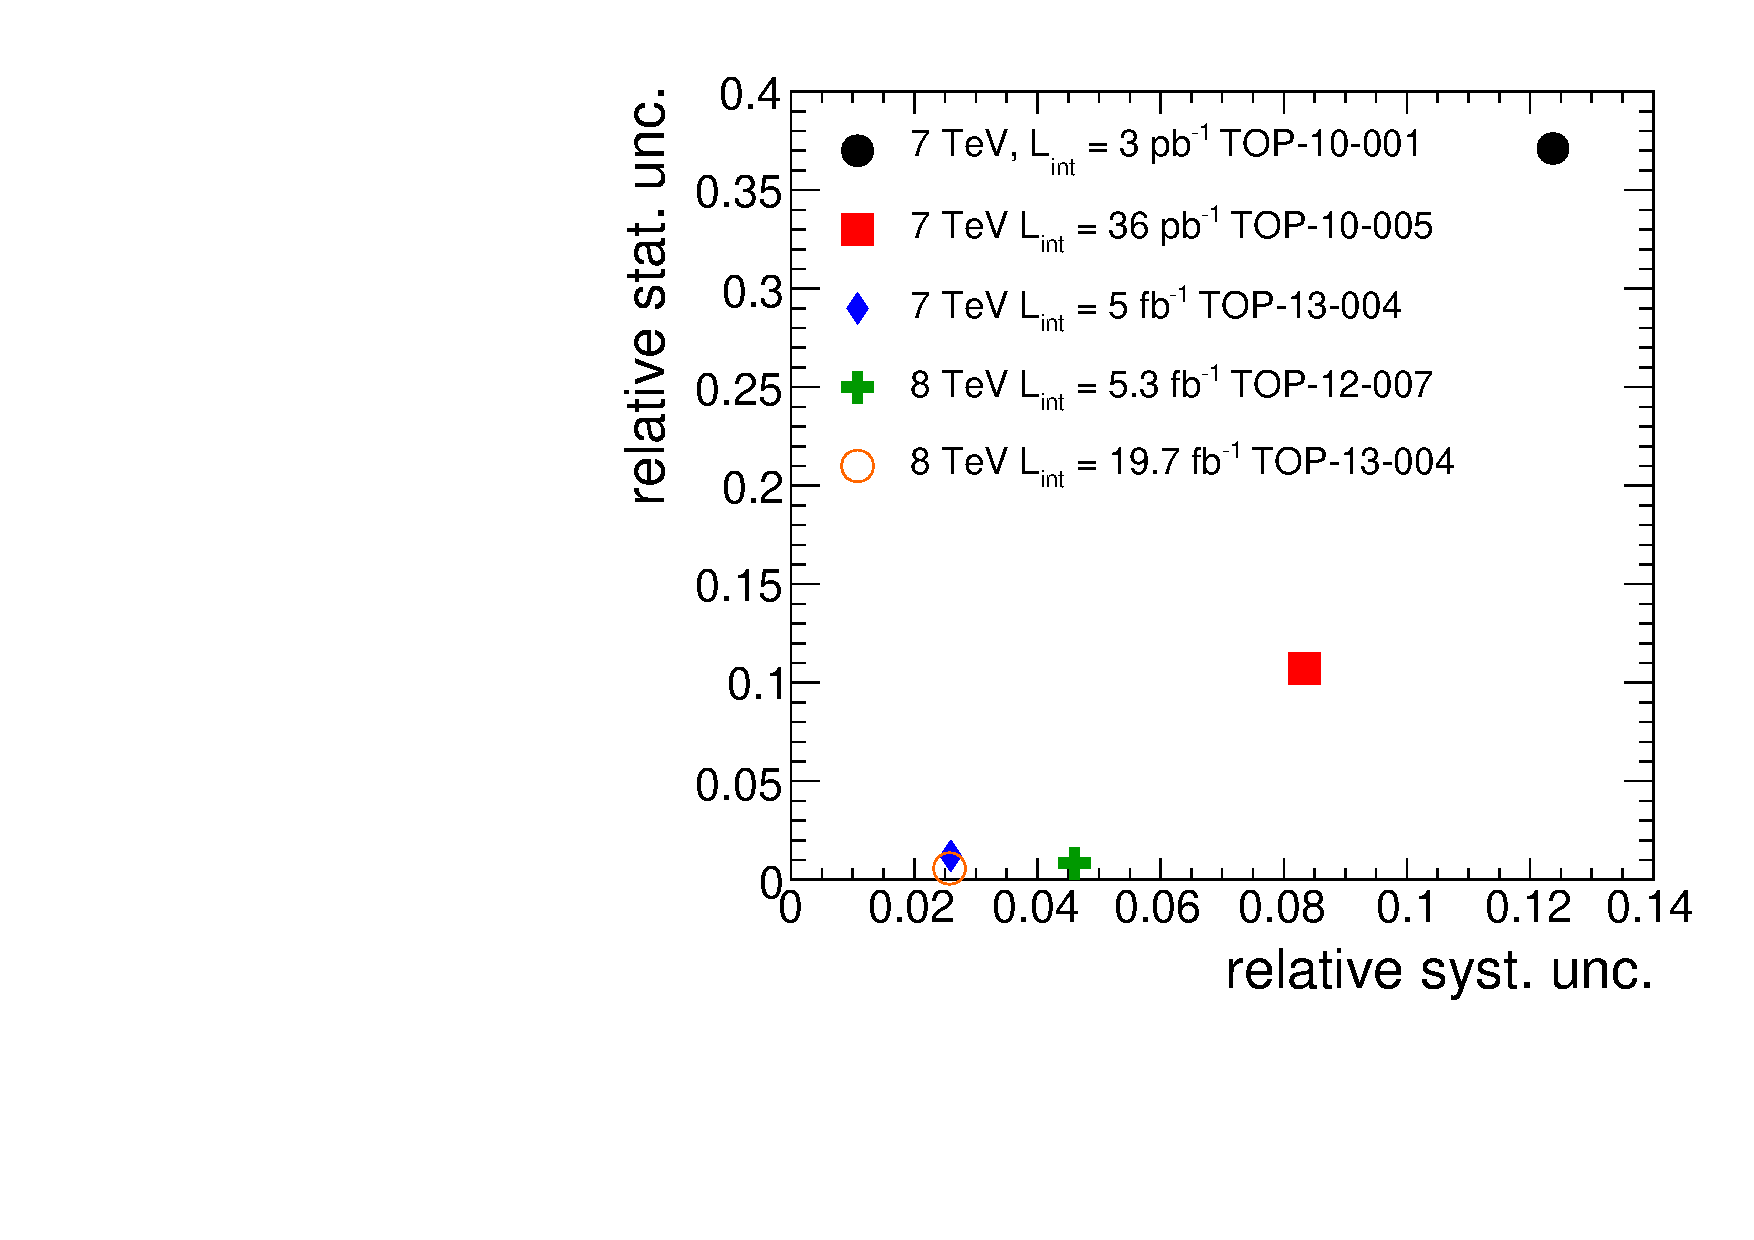
\includegraphics[width= 0.43\textwidth]{figures/top/topToLLXSecUncertaintiesPP.pdf}
  \caption{Evolution of statistical an systematic uncertainty of top pair cross section measurements in the fully leptonic channel in pp collisions at 7 and 8 TeV.
  }
\label{fig:ttStatSyst}
\end{center}
\end{figure}

\section*{Summary}

At 20--30 nb$^{-1}$, the splitting of
the run between 5.02 and 8.16 TeV would not be meaningful anymore since the same level of 
sensitivity can be achieved by simply running at 5.02 TeV for the entire run period.

\bibliography{theNote}
\bibliographystyle{plain}

\clearpage

\end{document}


